\documentclass[11pt,a4paper]{article}
\usepackage[utf8]{inputenc}
\usepackage[T1]{fontenc}
\usepackage[margin=2.4cm]{geometry}
\usepackage{amsmath,amssymb,amsthm,mathtools}
\usepackage{booktabs,array,enumitem}
\usepackage{xcolor}
\usepackage{tikz}
\usetikzlibrary{arrows.meta,positioning,calc,fit,matrix,shapes.geometric,decorations.pathreplacing,backgrounds}
\usepackage{pgfplots}
\usepgfplotslibrary{groupplots}
\pgfplotsset{compat=1.16}
\usepackage[most]{tcolorbox}
\usepackage[hidelinks]{hyperref}
\usepackage{float}
\usepackage{caption}
\captionsetup{font=small,labelfont=bf}

% ---------- macros ----------
\newcommand{\R}{\mathbb{R}}
\DeclareMathOperator{\softmax}{softmax}
\DeclareMathOperator{\LN}{LayerNorm}
\DeclareMathOperator{\MHA}{MHA}
\DeclareMathOperator{\SA}{SA}
\DeclareMathOperator{\CA}{CA}
\DeclareMathOperator{\argmax}{arg\,max}
\newcommand{\slides}[1]{\par\nopagebreak\noindent{\normalfont\small\emph{(slides #1)}}\par\nopagebreak\vspace{2pt}}

% ---------- theorem-like boxes ----------
\theoremstyle{definition}
\newtheorem{definition}{Definition}[section]
\newtheorem{example}[definition]{Example}
\newtheorem{algorithm}[definition]{Algorithm}
\theoremstyle{plain}
\newtheorem{lemma}[definition]{Lemma}
\newtheorem{theorem}[definition]{Theorem}
\newtheorem{proposition}[definition]{Proposition}
\newtheorem{corollary}[definition]{Corollary}

\tcbset{thmbox/.style={breakable,enhanced jigsaw,boxrule=0.6pt,arc=2pt,left=6pt,right=6pt,top=4pt,bottom=4pt,before skip=8pt,after skip=8pt}}
\tcolorboxenvironment{definition}{thmbox,colback=gray!6,colframe=gray!60!black}
\tcolorboxenvironment{example}{thmbox,colback=orange!5,colframe=orange!60!black}
\tcolorboxenvironment{algorithm}{thmbox,colback=green!5,colframe=green!40!black}
\tcolorboxenvironment{lemma}{thmbox,colback=red!4,colframe=red!50!black}
\tcolorboxenvironment{theorem}{thmbox,colback=red!4,colframe=red!50!black}
\tcolorboxenvironment{proposition}{thmbox,colback=red!4,colframe=red!50!black}
\tcolorboxenvironment{corollary}{thmbox,colback=red!4,colframe=red!50!black}

\newtcolorbox{intuition}{breakable,enhanced jigsaw,colback=blue!5,colframe=blue!60!black,
  coltitle=white,fonttitle=\bfseries,title=Intuition,boxrule=0.6pt,arc=2pt,
  before skip=6pt,after skip=10pt}

% ---------- blank photo slot ----------
\newcommand{\photoslot}[3]{% #1 slide, #2 height, #3 caption
  \begin{figure}[ht]\centering
  \begin{tikzpicture}
    \draw[dashed,thick,gray] (0,0) rectangle (0.85\textwidth,#2);
    \node[align=center,gray] at (0.425\textwidth,#2/2) {\textbf{[ Insert image here ]}\\[2pt]Take it from \textbf{slide #1} of the deck};
  \end{tikzpicture}
  \caption{#3}
  \end{figure}}

% ---------- TikZ styles ----------
\tikzset{
  tok/.style={draw,rounded corners=1.5pt,minimum height=6.5mm,minimum width=9mm,inner sep=2pt,font=\small,fill=white},
  box/.style={draw,rounded corners=2pt,minimum height=7mm,inner sep=4pt,font=\small,align=center,fill=white},
  blk/.style={draw,rounded corners=2pt,minimum height=7mm,minimum width=22mm,inner sep=3pt,font=\small,align=center},
  arr/.style={-{Stealth[length=2mm]},thick},
  lbl/.style={font=\scriptsize,gray!50!black},
}

\title{\textbf{Transformer (Attention-Based) Models}\\[2pt]\large Lecture notes -- Neural Networks 2024/2025}
\author{Notes based on the slides by S.\ Scardapane (Sapienza University of Rome)}
\date{}

\begin{document}
\maketitle
\tableofcontents

%==========================================================
\section*{About these notes}
\addcontentsline{toc}{section}{About these notes}
These notes follow the flow of the slide deck \emph{Transformer (attention-based) models} (66 slides). Section and subsection titles reuse the slide titles, each tagged with its slide range. The slides declare themselves an abridged version of Chapters 9--11 of \emph{Alice's Adventures in a Differentiable Wonderland}; the formal statements and proofs below are written out here at the point where the slides introduce each topic. Figures are redrawn from the slide captions and text as original TikZ/pgfplots graphics; the few images that cannot be reproduced are left as blank slots that say which slide to take them from.

\medskip
\noindent\textbf{Conventions.} Sequences are stored as matrices $X\in\R^{n\times d}$ ($n$ tokens, one per row, each of dimension $d$). Row vectors and column vectors are used as in the slides: $q_i=W_q^\top x_i$ is the $i$-th \emph{row} of $Q=XW_q$. \texttt{softmax} is always applied \emph{row by row} unless said otherwise.

\begin{intuition}
The whole story in one paragraph: convolutions only look at a fixed small neighbourhood, so they cannot relate far-apart tokens in one step. A transformer lets \emph{every} token look at \emph{every other} token, with weights computed from the content of the tokens themselves (attention). This freedom costs two things that the rest of the notes deal with: attention is blind to order (so we must inject positions) and it is quadratic in the sequence length.
\end{intuition}

%==========================================================
\section{Moving beyond convolutional layers}\slides{3--5}

\subsection{The problem of convolutions}\slides{3}
Convolutional layers embed the assumption of \emph{locality}: an output depends only on a small window of the input. This is not always optimal. In text, audio, graphs, etc., dependencies can be \textbf{sparse}, \textbf{long-range} and possibly \textbf{dynamic} (they depend on the data, not just on the position).

\begin{example}[Same relation, different distance]
In ``the cat is on the table'' and ``the cat, which belonged to my mother, is on the table'' the relation between \emph{cat} and \emph{is} is the same, but their relative position changes from 1 to 6.
\end{example}

\begin{figure}[H]
\centering
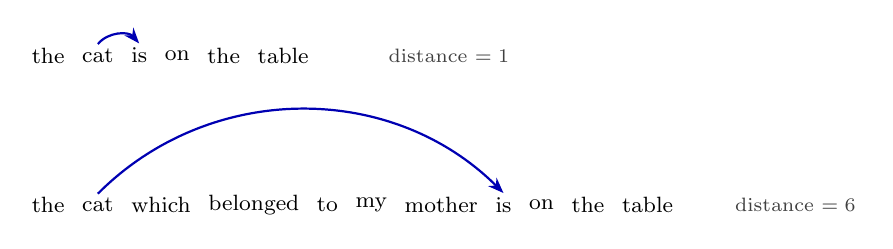
\begin{tikzpicture}[w/.style={font=\footnotesize,inner sep=1.5pt}]
% short sentence
\node[w] (a1) at (0,1.9) {the};
\node[w,right=3pt of a1] (a2) {cat};
\node[w,right=3pt of a2] (a3) {is};
\node[w,right=3pt of a3] (a4) {on};
\node[w,right=3pt of a4] (a5) {the};
\node[w,right=3pt of a5] (a6) {table};
\draw[arr,blue!70!black] (a2.north) to[bend left=50] (a3.north);
\node[lbl,anchor=west] at (4.2,1.9) {distance $=1$};
% long sentence
\node[w] (b1) at (0,0) {the};
\node[w,right=3pt of b1] (b2) {cat};
\node[w,right=3pt of b2] (b3) {which};
\node[w,right=3pt of b3] (b4) {belonged};
\node[w,right=3pt of b4] (b5) {to};
\node[w,right=3pt of b5] (b6) {my};
\node[w,right=3pt of b6] (b7) {mother};
\node[w,right=3pt of b7] (b8) {is};
\node[w,right=3pt of b8] (b9) {on};
\node[w,right=3pt of b9] (b10) {the};
\node[w,right=3pt of b10] (b11) {table};
\draw[arr,blue!70!black] (b2.north) to[bend left=45] (b8.north);
\node[lbl,anchor=west] at (8.6,0) {distance $=6$};
\end{tikzpicture}
\caption{Original toy illustration: the same subject--verb relation (arrow) spans a different number of positions. A kernel of size $k=3$ captures the first but not the second.}
\end{figure}

\begin{intuition}
A convolution is like reading through a small window sliding along the sentence. If the subject and its verb are never inside the same window, no single layer can connect them; you would have to stack many layers (a deep receptive field) or enlarge the window (many parameters). Attention instead lets the verb ``reach out'' directly to the subject, wherever it is.
\end{intuition}

\subsection{Transformers}\slides{4}
In 2017 a new architecture, the \textbf{transformer}, was proposed for text processing (Vaswani et al., 2017) and was then extended to most other modalities. The original model was an encoder-decoder model for NLP; today similar models are widespread in computer vision, audio, biology, etc.

The core is a new layer, \textbf{multi-head attention (MHA)}. It replaces the assumption of locality with a more general notion of \emph{(soft) sparsity of interactions}: each token interacts mostly with a few others, chosen dynamically.

\subsection{Transformers have better scaling laws}\slides{5}
Empirically, transformers keep improving as data and model size grow by orders of magnitude, more so than other architectures (the slide shows results from the Big Transfer, BiT, study on large-scale pre-training for vision).

\begin{figure}[H]
	\centering
	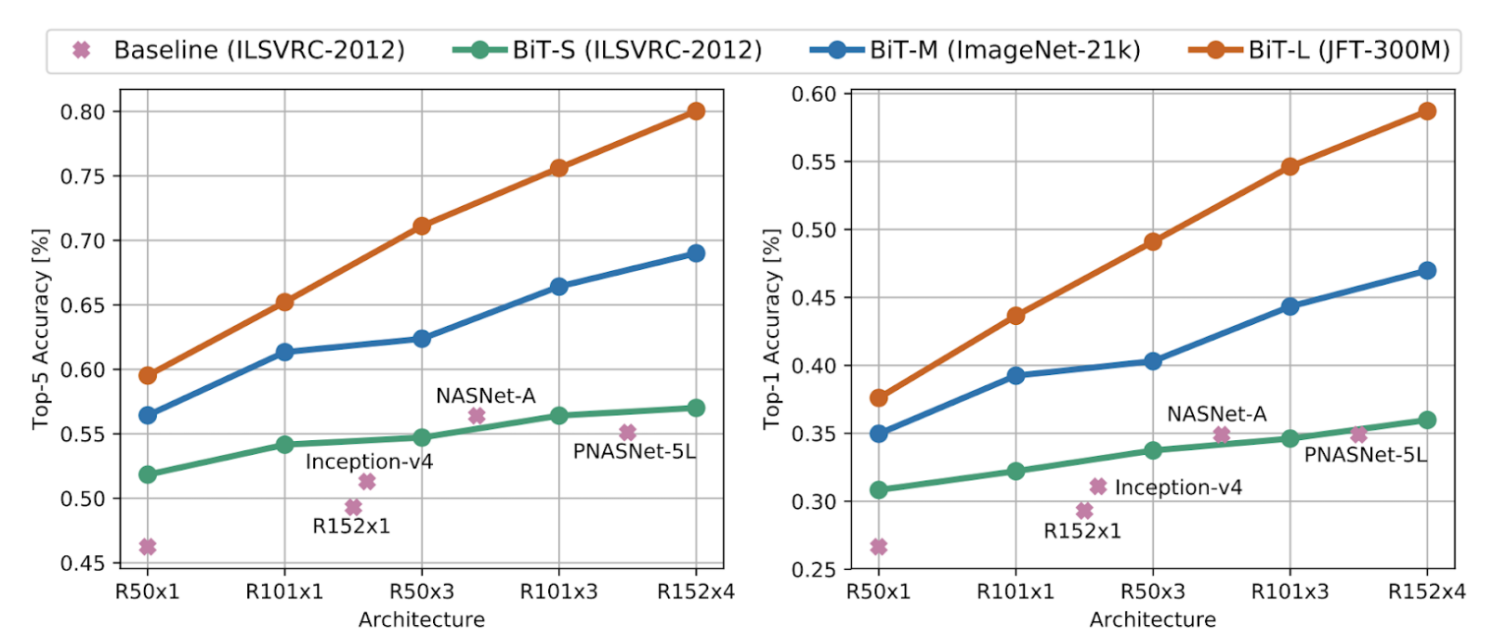
\includegraphics[width=1.0\linewidth]{1795435487177.png}
	\caption{Transformers have better scaling laws. Performance of the models as the pre-training dataset grows (from the Google AI Blog post \emph{Open-Sourcing BiT: Exploring Large-Scale Pre-training for Computer Vision}).}\label{fig:1795435487177}
\end{figure}

\begin{intuition}
``Scaling law'' means: if you plot accuracy against the amount of pre-training data (log scale), some architectures flatten out early, while transformers keep climbing. This is why they became the default when very large datasets are available.
\end{intuition}

%==========================================================
\section{Text tokenization}\slides{6--12}

\subsection{Handling text data}\slides{6}
Text must be preprocessed before a neural network can handle it. At the very least we perform two operations:
\begin{enumerate}[nosep]
\item \textbf{Tokenize} the text, splitting it into basic units (tokens) that form a sequence;
\item \textbf{Embed} each token (one or more characters), i.e.\ convert it into numerical features.
\end{enumerate}

\begin{definition}[Token sequence and embedding matrix]
Let $\mathcal V$ be a vocabulary of $V$ tokens. A text is tokenized into a sequence $(c_1,\dots,c_n)$ with $c_i\in\mathcal V$. An \emph{embedding} maps each $c_i$ to a vector $x_i\in\R^d$; stacking the vectors gives the matrix $X\in\R^{n\times d}$ that is fed to the network.
\end{definition}

The slides ignore many other preprocessing steps (stemming, stop-word removal, \dots).

\subsection{Text tokenization}\slides{7}
Tokenization can be done at several levels, usually by an external library (e.g.\ Spacy).

\begin{figure}[H]
\centering
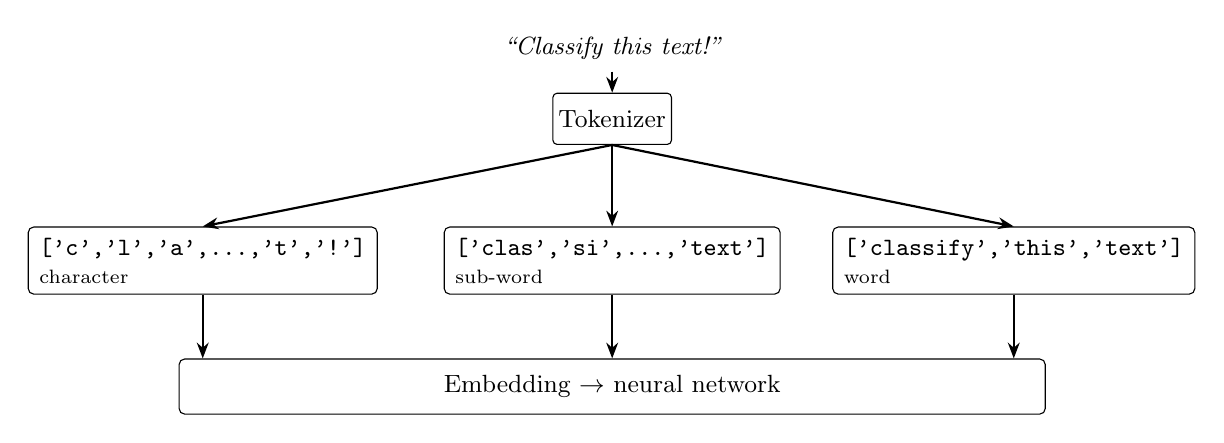
\begin{tikzpicture}
\node[font=\small\itshape] at (0,3.3) {``Classify this text!''};
\node[tok,minimum width=14mm] (t) at (0,2.4) {Tokenizer};
\draw[arr] (0,3.0) -- (t.north);
\node[box,align=left] (c) at (-5.2,0.6) {\texttt{['c','l','a',\dots,'t','!']}\\[-1pt]{\scriptsize character}};
\node[box,align=left] (s) at (0,0.6) {\texttt{['clas','si',\dots,'text']}\\[-1pt]{\scriptsize sub-word}};
\node[box,align=left] (w) at (5.1,0.6) {\texttt{['classify','this','text']}\\[-1pt]{\scriptsize word}};
\draw[arr] (t.south) -- (c.north);
\draw[arr] (t.south) -- (s.north);
\draw[arr] (t.south) -- (w.north);
\node[box,minimum width=11cm] (e) at (0,-1) {Embedding $\rightarrow$ neural network};
\draw[arr] (c.south) -- (c |- e.north);
\draw[arr] (s.south) -- (s |- e.north);
\draw[arr] (w.south) -- (w |- e.north);
\end{tikzpicture}
\caption{Tokenization at character, sub-word and word level, followed by the embedding step (redrawn from slide 7).}
\end{figure}

\subsection{The importance of tokenization}\slides{8}
Tokenization determines what the network will ``see''. Version 15 of Unicode has almost 150k symbols, which can be combined in many forms (numbers, dates, function names, \dots). \textbf{Sub-word} tokenization is very common, especially when the sub-words are \emph{learned} from large text corpora (e.g.\ byte pair encoding, BPE).

\begin{intuition}
Characters give tiny vocabularies but very long sequences; words give short sequences but huge (and open-ended) vocabularies with many unseen words. Sub-words are the compromise: frequent words stay whole, rare ones are split in reusable pieces (``clas'' + ``si'' + \dots).
\end{intuition}

\subsection{One-hot encoding}\slides{9}
The simplest vector embedding is a one-hot encoding with respect to a predefined dictionary:
\begin{itemize}[nosep]
\item \textbf{Character level:} a 1-of-$C$ binary vector, $C$ = number of allowed characters.
\item \textbf{Sub-word/word level:} the same, with respect to a fixed vocabulary of sub-words/words.
\item \textbf{Sentence level:} sum the one-hot encodings of the tokens (\emph{bag-of-words}).
\end{itemize}

\begin{proposition}[Geometry of one-hot vectors]\label{prop:onehot}
Let $e_a,e_b\in\{0,1\}^V$ be one-hot vectors of two distinct tokens. Then $\|e_a-e_b\|_2=\sqrt 2$ and $e_a^\top e_b=0$. For identical tokens the distance is $0$.
\end{proposition}
\begin{proof}
$e_a-e_b$ has exactly two non-zero entries, $+1$ and $-1$, so its squared norm is $2$. The inner product vanishes because the two ones are in different positions.
\end{proof}

\begin{intuition}
In a one-hot space every word is equally far from every other: ``cat'' is as far from ``dog'' as from ``carburetor'' (distance $\sqrt2\approx1.41$). The representation carries identity but no \emph{meaning}.
\end{intuition}

\subsection{Dense embeddings}\slides{10}
A more general solution is to \emph{learn} the embeddings:
\begin{enumerate}[nosep]
\item For every possible token $c$, randomly initialize a fixed-size vector $v_c$.
\item During training, substitute each token of the sequence with its vector (look-up).
\item Optimize the $v_c$ together with the other parameters by gradient descent.
\end{enumerate}

\begin{proposition}[Look-up is a linear map on one-hot vectors]\label{prop:lookup}
Let $E\in\R^{V\times d}$ be the matrix whose $c$-th row is $v_c$. Then $e_c^\top E=v_c^\top$. Moreover, for a loss $\mathcal L$ the gradient with respect to $E$ has non-zero rows only for the tokens that actually appear in the input.
\end{proposition}
\begin{proof}
$e_c^\top E$ selects the $c$-th row of $E$. For the sequence $(c_1,\dots,c_n)$, $X=OE$ with $O$ the $n\times V$ one-hot matrix, so $\partial\mathcal L/\partial E=O^\top\,\partial\mathcal L/\partial X$, whose $c$-th row is $\sum_{i:c_i=c}\partial\mathcal L/\partial x_i$ and is zero if $c$ never appears.
\end{proof}

\begin{intuition}
An embedding layer is a big table with one learnable row per token. Training a sentence only edits the rows of the words it contains. Words used in similar contexts receive similar gradients, so their rows drift together.
\end{intuition}

\subsection{Visualizing the embedding procedure}\slides{11}
\begin{figure}[H]
\centering
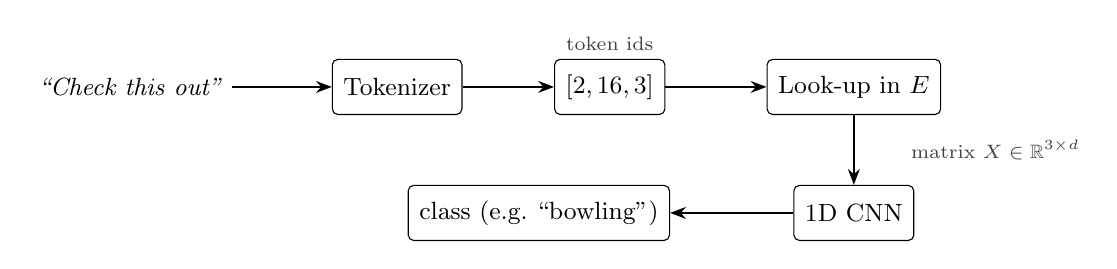
\begin{tikzpicture}[x=1cm,y=1cm]
\node[font=\small\itshape,align=center] (txt) at (0,0) {``Check this out''};
\node[box] (tk) at (3.4,0) {Tokenizer};
\node[box] (id) at (6.1,0) {$[2,16,3]$};
\node[box] (em) at (9.2,0) {Look-up in $E$};
\node[box] (cnn) at (9.2,-1.6) {1D CNN};
\node[box] (out) at (5.2,-1.6) {class (e.g.\ ``bowling'')};
\draw[arr] (txt) -- (tk); \draw[arr] (tk) -- (id); \draw[arr] (id) -- (em);
\draw[arr] (em) -- (cnn); \draw[arr] (cnn) -- (out);
\node[lbl] at (6.1,0.55) {token ids};
\node[lbl] at (11.0,-0.8) {matrix $X\in\R^{3\times d}$};
\end{tikzpicture}
\caption{Using custom (trainable) embeddings for text classification: the token ids index rows of a learnable table, and the resulting matrix is processed by a standard network (here a 1D CNN). Redrawn from slide 11.}
\end{figure}

\subsection{Dense vs.\ sparse embeddings}\slides{12}
One-hot encodings are \emph{sparse} (most values are $0$) and not very informative: the distance between any two of them is either $0$ or $\sqrt2$ (Proposition~\ref{prop:onehot}). Trained embeddings can capture rich semantics of the data, reflected in the possibility of doing \emph{algebraic manipulations} on the embeddings themselves. However, they can also capture \textbf{biases} of the data (Bolukbasi et al., 2016).

\begin{figure}[H]
\centering
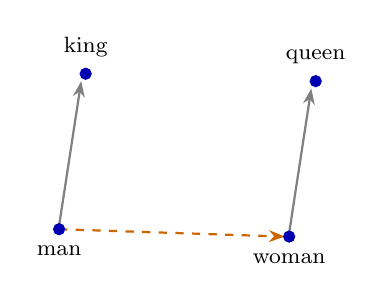
\begin{tikzpicture}
\begin{axis}[width=7.2cm,height=6cm,axis lines=none,xmin=-0.5,xmax=4.5,ymin=-0.5,ymax=4.2,clip=false]
\addplot[only marks,mark=*,mark size=2pt,blue!70!black] coordinates {(0.6,0.8) (0.9,2.9) (3.2,0.7) (3.5,2.8)};
\node[font=\footnotesize,anchor=north] at (axis cs:0.6,0.7) {man};
\node[font=\footnotesize,anchor=south] at (axis cs:0.9,3.0) {king};
\node[font=\footnotesize,anchor=north] at (axis cs:3.2,0.6) {woman};
\node[font=\footnotesize,anchor=south] at (axis cs:3.5,2.9) {queen};
\draw[arr,gray] (axis cs:0.6,0.85) -- (axis cs:0.85,2.8);
\draw[arr,gray] (axis cs:3.2,0.75) -- (axis cs:3.45,2.7);
\draw[arr,orange!80!black,dashed] (axis cs:0.6,0.8) -- (axis cs:3.15,0.7);
\end{axis}
\end{tikzpicture}
\caption{Hand-placed, purely illustrative 2D picture of the classic analogy: the offset man$\to$king is roughly the offset woman$\to$queen, so $\text{king}-\text{man}+\text{woman}\approx\text{queen}$. No real embeddings are plotted.}
\end{figure}

\begin{intuition}
Dense embeddings turn ``meaning'' into geometry: directions in the space correspond to concepts (gender, plural, tense, \dots). The flip side: if the training text associates certain professions with one gender, that association becomes a direction in the space too.
\end{intuition}

%==========================================================
\section{Self-attention}\slides{13--26}

\subsection{Moving beyond locality}\slides{13}
Consider a 1D sequence $x_1,\dots,x_n$ with $x_i\in\R^d$; each element is a \textbf{token} and $d$ is the embedding dimension.

\begin{definition}[1D convolutional layer]
Ignoring padding, a 1D convolution with kernel size $k$ is
\begin{equation}\label{eq:conv}
h_i=\sum_{j=-k}^{k}W_j\,x_{i+j},
\end{equation}
where $W$ is the kernel tensor, i.e.\ $2k{+}1$ matrices $W_j\in\R^{d\times d}$ (the slide writes the shape as $(2k,d,d)$).
\end{definition}

The number of parameters grows \emph{linearly} in $k$: $(2k+1)d^2$. We want to remove the locality assumption while keeping parameter efficiency.

\subsection{Continuous convolutions}\slides{14}
Instead of one free matrix per shift, learn a trainable block $g:\mathbb N\to\R^{d\times d}$ that \emph{generates} the kernel from the shift.

\begin{definition}[Continuous convolution]
\begin{equation}\label{eq:contconv}
h_i=\sum_{j=-i+1}^{\,n-i}g(j)\,x_{i+j},
\end{equation}
with a single trainable function $g$ (e.g.\ a small network) taking the shift $j$ as input.
\end{definition}
These work well on image-like data of variable sizes and resolutions (Romero et al., 2022).

\begin{intuition}
Instead of storing a lookup table of weights (one per offset), we store a \emph{recipe} $g$ that can produce a weight for any offset, even very far away. Number of parameters = size of $g$, independent of how long the sequence is. But the weight still depends only on the \emph{offset} $j$, not on what the tokens are.
\end{intuition}

\subsection{Non-local neural networks}\slides{15}
The previous model handles non-locality, but dependencies are still \emph{regular}: they depend only on $j$. We make it more general by letting them depend on the \emph{values} of the tokens.

\begin{definition}[Non-local layer]
\begin{equation}\label{eq:nonlocal}
h_i=\sum_{j=1}^{n}\alpha(x_i,x_j)\,x_j .
\end{equation}
\end{definition}
(Wang et al., 2018). With a proper choice of the weighting function $\alpha(\cdot,\cdot)$ we obtain the MHA layer.

\subsection{Schematic depiction}\slides{16}
\begin{figure}[H]
\centering
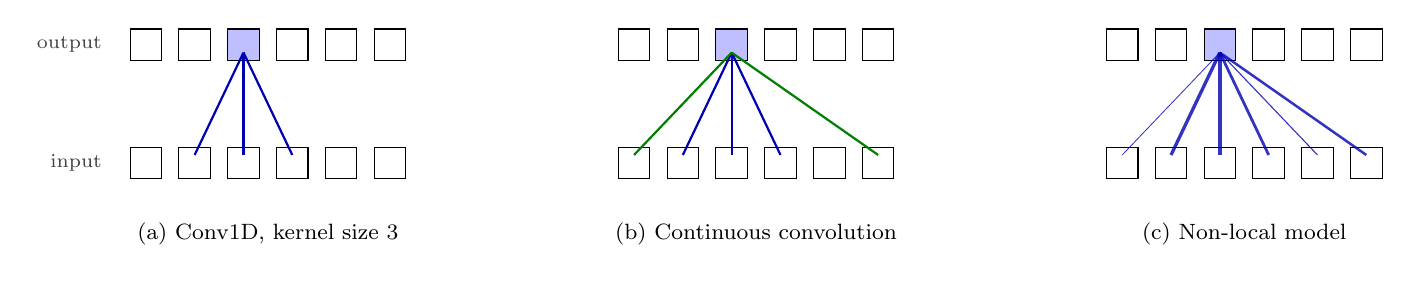
\begin{tikzpicture}[x=0.62cm,y=1cm]
\newcommand{\row}{%
  \foreach \i in {1,...,6}{\node[draw,minimum size=4mm,inner sep=0] at (\i,0) {}; \node[draw,minimum size=4mm,inner sep=0] at (\i,1.5) {};}}
% (a)
\begin{scope}
 \row
 \node[draw,fill=blue!25,minimum size=4mm,inner sep=0] at (3,1.5) {};
 \foreach \j in {2,3,4}{\draw[blue!70!black,thick] (3,1.4)--(\j,0.1);}
 \node[font=\footnotesize,align=center] at (3.5,-0.9) {(a) Conv1D, kernel size 3};
\end{scope}
% (b)
\begin{scope}[xshift=6.2cm]
 \row
 \node[draw,fill=blue!25,minimum size=4mm,inner sep=0] at (3,1.5) {};
 \foreach \j in {2,3,4}{\draw[blue!70!black,thick] (3,1.4)--(\j,0.1);}
 \draw[green!50!black,thick] (3,1.4)--(1,0.1);
 \draw[green!50!black,thick] (3,1.4)--(6,0.1);
 \node[font=\footnotesize,align=center] at (3.5,-0.9) {(b) Continuous convolution};
\end{scope}
% (c)
\begin{scope}[xshift=12.4cm]
 \row
 \node[draw,fill=blue!25,minimum size=4mm,inner sep=0] at (3,1.5) {};
 \foreach \j/\w in {1/0.3,2/1.2,3/1.6,4/1.0,5/0.4,6/0.9}{\draw[blue!70!black,line width=\w pt,opacity=0.8] (3,1.4)--(\j,0.1);}
 \node[font=\footnotesize,align=center] at (3.5,-0.9) {(c) Non-local model};
\end{scope}
\node[lbl,anchor=east] at (0.3,0) {input};
\node[lbl,anchor=east] at (0.3,1.5) {output};
\end{tikzpicture}
\caption{Short-term (blue) and long-term (green) interactions for one output token (shaded). (a)~Conv1D: short-term connections have trainable weights, long-term ones are removed. (b)~Continuous convolution: both connection types exist, their weights are given by $g(\cdot)$ of the shift (e.g.\ $g(-1)$, $g(2)$). (c)~Non-local model: every connection exists and its weight (line width) depends on the tokens' similarity. Redrawn from slide 16.}
\end{figure}

\subsection{Choosing the weighting function}\slides{17}
We make a few assumptions to simplify the layer:
\begin{itemize}[nosep]
\item The output of $\alpha$ is a \textbf{scalar} (not a matrix): the \emph{attention scoring function}; its outputs are the \emph{attention scores} of token $i$.
\item For each token the attention scores are \textbf{normalized in the simplex} (positive, summing to one): every token has a ``budget'' of attention to allocate, so increasing one score necessarily decreases the others.
\end{itemize}

\begin{definition}[Attention weights]
Given scores $s_{ij}=\alpha(x_i,x_j)\in\R$, the attention weights of token $i$ are
\[
a_{ij}=\softmax_j(s_{i\cdot})=\frac{e^{s_{ij}}}{\sum_{l=1}^{n}e^{s_{il}}},\qquad a_{ij}>0,\quad\sum_j a_{ij}=1 .
\]
\end{definition}

\begin{proposition}[Attention is a convex combination]\label{prop:convex}
For every $i$, the output $h_i=\sum_j a_{ij}x_j$ lies in the convex hull of $\{x_1,\dots,x_n\}$.
\end{proposition}
\begin{proof}
The coefficients $a_{ij}$ are positive and sum to one, which is the definition of a convex combination.
\end{proof}

\begin{intuition}
Think of each token as having $100\%$ of its attention to distribute. If it gives $70\%$ to ``cat'', only $30\%$ is left for everything else. The output is therefore a \emph{weighted average} of the tokens, never something outside their range, and it is ``sparse in a soft sense'' when a few weights dominate.
\end{intuition}

\subsection{Attention layer}\slides{18}
There are many choices for the attention function; commonly we use the \textbf{normalized dot product}
\[
\alpha(x_i,x_j)=\frac{1}{\sqrt d}\,x_i^\top x_j ,
\]
because it is fast and efficient to parallelize. Putting everything together (for a single token):
\begin{equation}\label{eq:attn-nolearn}
h_i=\sum_{j=1}^{n}\softmax_j\!\Big(\tfrac{1}{\sqrt d}x_j^\top x_i\Big)\,x_j .
\end{equation}

\paragraph{Why the extra factor $\sqrt d$?}
\begin{lemma}[Variance of a dot product]\label{lem:var}
Let $x,y\in\R^{q}$ have independent entries sampled from $\mathcal N(0,\sigma^2)$. Then $\mathbb E[x^\top y]=0$ and $\operatorname{Var}(x^\top y)=q\,\sigma^4$. Hence $\operatorname{Var}\!\big(x^\top y/\sqrt q\big)=\sigma^4$ for every $q$.
\end{lemma}
\begin{proof}
$x^\top y=\sum_{l=1}^{q}x_ly_l$. Each product has mean $0$ and variance $\mathbb E[x_l^2]\,\mathbb E[y_l^2]=\sigma^4$, and the $q$ products are independent, so the variances add up to $q\sigma^4$. Dividing by $\sqrt q$ divides the variance by $q$.
\end{proof}
(The slide's ``$\sigma^4$'' is the variance of a single coordinate product; the full dot product has $q$ of them.)

\begin{example}[Softmax saturation]\label{ex:sat}
Take $q=64$ and $\sigma=1$. Unscaled scores have standard deviation $\sqrt{64}=8$, so typical scores look like $(8,0,-8)$ and $\softmax(8,0,-8)\approx(0.9997,\,0.0003,\,0.0000)$: almost one-hot. After dividing by $\sqrt{64}=8$ the scores are $(1,0,-1)$ and $\softmax(1,0,-1)\approx(0.665,\,0.245,\,0.090)$: a healthy, spread-out distribution.
\end{example}

\begin{figure}[H]
\centering
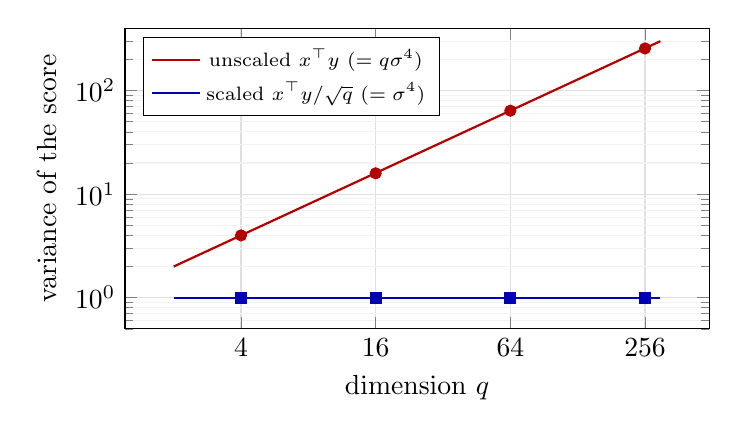
\begin{tikzpicture}
\begin{axis}[width=9cm,height=5.4cm,xmode=log,ymode=log,log basis x=2,xlabel={dimension $q$},ylabel={variance of the score},
  legend pos=north west,legend style={font=\scriptsize},grid=both,minor grid style={gray!10},major grid style={gray!25},xtick={4,16,64,256},xticklabels={4,16,64,256},ymin=0.5,ymax=400]
\addplot[domain=2:300,samples=30,thick,red!70!black] {x};
\addlegendentry{unscaled $x^\top y$ ($=q\sigma^4$)}
\addplot[domain=2:300,samples=2,thick,blue!70!black] {1};
\addlegendentry{scaled $x^\top y/\sqrt q$ ($=\sigma^4$)}
\addplot[only marks,mark=*,red!70!black] coordinates {(4,3.996) (16,15.90) (64,63.95) (256,255.3)};
\addplot[only marks,mark=square*,blue!70!black] coordinates {(4,0.999) (16,0.994) (64,0.999) (256,0.997)};
\end{axis}
\end{tikzpicture}
\caption{Lemma~\ref{lem:var} with $\sigma=1$: lines are the exact variances; markers are Monte-Carlo estimates ($2\cdot10^5$ random pairs per dimension) that I computed to double-check the lemma.}
\end{figure}

\begin{intuition}
Without scaling, the scores grow like $\sqrt q$ as vectors get longer. The softmax then behaves like an argmax (one token gets everything) and its gradient almost vanishes, so learning stalls. Dividing by $\sqrt q$ keeps the scores at a constant scale (std $\approx\sigma^2$) no matter how large the embedding is.
\end{intuition}

\subsection{Adding some parameters}\slides{19}
So far the layer has no trainable parameters. We first \emph{re-project} the input three times with trainable matrices:
\[
q_i=W_q^\top x_i,\qquad k_i=W_k^\top x_i,\qquad v_i=W_v^\top x_i ,
\]
called the \textbf{query}, \textbf{key} and \textbf{value} (the reason is explained shortly).

\begin{definition}[Self-attention (SA) layer]
\begin{equation}\label{eq:sa}
h_i=\sum_{j=1}^{n}\softmax_j\!\Big(\tfrac{1}{\sqrt q}\,q_i^\top k_j\Big)\,v_j .
\end{equation}
(The slide writes $1/\sqrt d$; in the vectorized version it is $1/\sqrt q$, the dimension of queries and keys. They coincide when $q=d$.)
\end{definition}

\subsection{Vectorized version}\slides{20}
Stack the $n$ input vectors into $X\in\R^{n\times d}$.

\begin{definition}[Vectorized SA]
\[
Q=XW_q,\quad K=XW_k,\quad V=XW_v,\qquad H=\softmax\!\Big(\frac{QK^\top}{\sqrt q}\Big)V ,
\]
with $W_q,W_k\in\R^{d\times q}$, $W_v\in\R^{d\times v}$, hence $Q,K\in\R^{n\times q}$ and $H\in\R^{n\times v}$. The hyper-parameters are $q$ and $v$.
\end{definition}

\begin{proposition}[Equivalence of the two forms]
Row $i$ of the vectorized $H$ equals $h_i$ in~\eqref{eq:sa}.
\end{proposition}
\begin{proof}
Row $i$ of $Q$ is $q_i^\top$ and row $j$ of $K$ is $k_j^\top$, so $(QK^\top)_{ij}=q_i^\top k_j$. The row-wise softmax gives $a_{ij}$. Row $i$ of $AV$ with $A=(a_{ij})$ is $\sum_j a_{ij}v_j^\top=h_i^\top$.
\end{proof}

When applied to a \emph{batch} (e.g.\ of sentences), the attention is computed independently for every element: a token only attends to tokens of its own sentence.

\begin{example}[A $3$-token toy computation]\label{ex:toy}
Let $d=q=v=2$, $W_q=W_k=W_v=I$ and
$X=\begin{psmallmatrix}1&0\\0&1\\1&1\end{psmallmatrix}$. Then
\[
\tfrac{1}{\sqrt2}QK^\top=\begin{pmatrix}0.71&0&0.71\\0&0.71&0.71\\0.71&0.71&1.41\end{pmatrix},\quad
A=\begin{pmatrix}0.40&0.20&0.40\\0.20&0.40&0.40\\0.25&0.25&0.50\end{pmatrix},\quad
H=AX\approx\begin{pmatrix}0.80&0.60\\0.60&0.80\\0.75&0.75\end{pmatrix}.
\]
For instance row~1 of $A$ is $\big(e^{0.71},e^{0},e^{0.71}\big)/5.06=(0.40,0.20,0.40)$.
\end{example}

\begin{figure}[H]
\centering
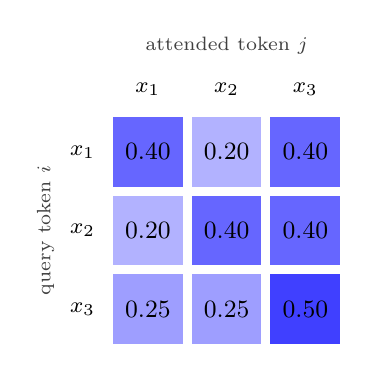
\begin{tikzpicture}[cell/.style={minimum size=9mm,inner sep=0,font=\small}]
\foreach \r/\c/\v/\p in {1/1/0.40/60,1/2/0.20/30,1/3/0.40/60,2/1/0.20/30,2/2/0.40/60,2/3/0.40/60,3/1/0.25/38,3/2/0.25/38,3/3/0.50/75}{
 \node[cell,fill=blue!\p!white,draw=white] at (\c,-\r) {\v};}
\foreach \i in {1,2,3}{\node[font=\footnotesize] at (\i,-0.2) {$x_\i$}; \node[font=\footnotesize,anchor=east] at (0.45,-\i) {$x_\i$};}
\node[lbl] at (2,0.35) {attended token $j$};
\node[lbl,rotate=90] at (-0.3,-2) {query token $i$};
\end{tikzpicture}
\caption{Attention matrix $A$ of Example~\ref{ex:toy}. Each row sums to one. Token $x_3=(1,1)$, which is similar to both others and has the largest norm, keeps $50\%$ of its attention for itself.}
\end{figure}

\begin{intuition}
$QK^\top$ is an $n\times n$ table of ``how much does token $i$ care about token $j$''. The softmax turns each row into percentages, and multiplying by $V$ mixes the value vectors in those percentages. In Example~\ref{ex:toy} token $x_1=(1,0)$ ends up as a blend of itself, of $x_2$ and of $x_3$, which is why its output $(0.80,0.60)$ now contains some of the second coordinate.
\end{intuition}

\subsection{Visualizing the attention operation}\slides{21}
\begin{figure}[H]
\centering
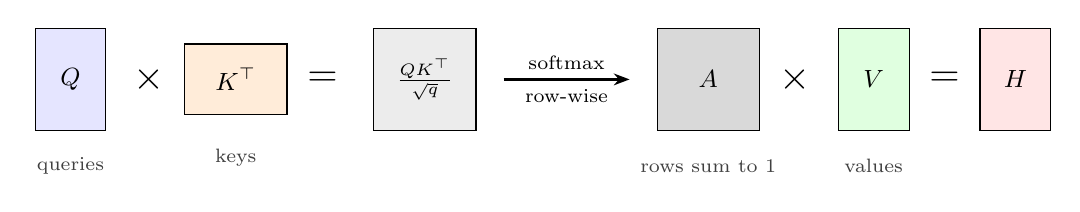
\begin{tikzpicture}[mat/.style={draw,minimum width=9mm,minimum height=13mm,font=\small,fill=white}]
\node[mat,fill=blue!10] (Q) at (0,0) {$Q$};
\node[font=\Large] at (1.0,0) {$\times$};
\node[mat,minimum width=13mm,minimum height=9mm,fill=orange!15] (K) at (2.1,0) {$K^\top$};
\node[font=\Large] at (3.2,0) {$=$};
\node[mat,minimum width=13mm,fill=gray!15] (S) at (4.5,0) {$\frac{QK^\top}{\sqrt q}$};
\draw[arr] (5.5,0) -- node[above,font=\scriptsize]{softmax} node[below,font=\scriptsize]{row-wise} (7.1,0);
\node[mat,minimum width=13mm,fill=gray!30] (A) at (8.1,0) {$A$};
\node[font=\Large] at (9.2,0) {$\times$};
\node[mat,fill=green!12] (V) at (10.2,0) {$V$};
\node[font=\Large] at (11.1,0) {$=$};
\node[mat,fill=red!10] (H) at (12.0,0) {$H$};
\node[lbl] at (0,-1.1) {queries};
\node[lbl] at (2.1,-1.0) {keys};
\node[lbl,align=center] at (8.1,-1.1) {rows sum to 1};
\node[lbl] at (10.2,-1.1) {values};
\end{tikzpicture}
\caption{The attention operation (initial projections omitted). Redrawn from slide 21.}
\end{figure}

\subsection{The dictionary analogy}\slides{22}
To understand the terminology, consider a Python dictionary \texttt{d = dict(...)}: a collection of key/value pairs $(k,v)$ such that for a query \texttt{d[q]} we get $v$ if $k=q$ is stored; otherwise an error or a default value is returned.

Consider instead a ``soft'' variant that \emph{always} returns a value: the value associated to the most similar key, even if no perfect match occurs. If keys, queries and values are vectors and similarity is the dot product, this is exactly SA with the softmax replaced by an argmax over rows.

\begin{definition}[Soft dictionary lookup]
Given keys $k_1,\dots,k_n$, values $v_1,\dots,v_n$ and a query $q$, the \emph{hard} lookup returns $v_{m}$ with $m=\argmax_j q^\top k_j$; the \emph{soft} lookup returns $\sum_j\softmax_j(q^\top k_j)\,v_j$.
\end{definition}

\begin{intuition}
\emph{Query} = what I am looking for; \emph{key} = the label on each drawer; \emph{value} = what is inside the drawer. A hard dictionary opens one drawer; attention opens all of them, a little bit each, in proportion to how well the label matches your request.
\end{intuition}

\subsection{Hard attention as a dictionary}\slides{23}
\begin{figure}[H]
\centering
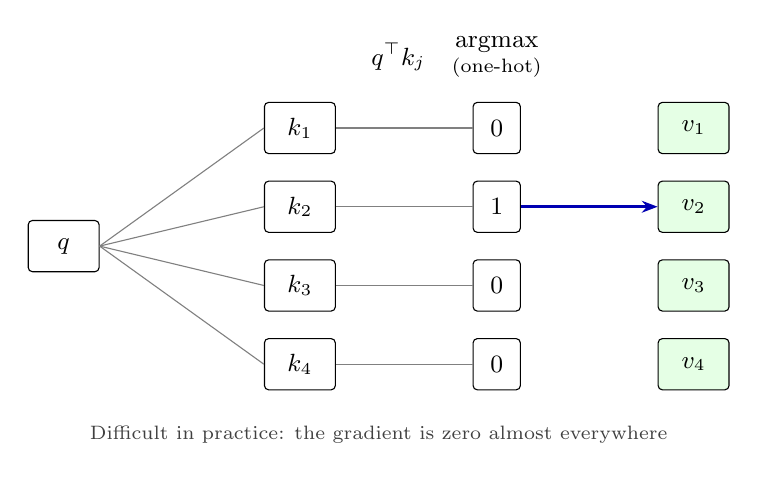
\begin{tikzpicture}
\node[tok] (q) at (0,0) {$q$};
\foreach \i/\y/\b in {1/1.5/0,2/0.5/1,3/-0.5/0,4/-1.5/0}{
 \node[tok] (k\i) at (3,\y) {$k_\i$};
 \node[tok,minimum width=6mm] (b\i) at (5.5,\y) {\b};
 \node[tok,fill=green!10] (v\i) at (8,\y) {$v_\i$};
 \draw[gray] (q.east) -- (k\i.west);
 \draw[gray] (k\i.east) -- (b\i.west);
}
\draw[blue!70!black,very thick,-{Stealth[length=2mm]}] (b2.east) -- (v2.west);
\node[font=\small,align=center] at (4.25,2.4) {$q^\top k_j$};
\node[font=\small,align=center] at (5.5,2.4) {argmax\\[-2pt]{\scriptsize(one-hot)}};
\node[lbl] at (4.0,-2.4) {Difficult in practice: the gradient is zero almost everywhere};
\end{tikzpicture}
\caption{Hard attention is a dictionary with associative recall: the query best matches $k_2$, the one-hot vector selects $v_2$. Redrawn from slide 23 (the slide notes that this is difficult in practice).}
\end{figure}

\begin{proposition}[Soft $\to$ hard as the temperature goes to $0$]\label{prop:temp}
For $z\in\R^n$ and $\beta>0$, let $m=|\argmax_l z_l|$. As $\beta\to\infty$, $\softmax(\beta z)_k\to 1/m$ if $k\in\argmax_l z_l$ and $\to0$ otherwise.
\end{proposition}
\begin{proof}
Write $\softmax(\beta z)_k=1\big/\sum_l e^{\beta(z_l-z_k)}$. If $z_k=\max z$, the $m$ terms with $z_l=z_k$ equal $1$ and all others tend to $0$, so the sum tends to $m$. If $z_k<\max z$, the term of any maximizer is $e^{\beta(\max z-z_k)}\to\infty$, so the softmax tends to $0$.
\end{proof}

\begin{proposition}[Exact recall with orthogonal keys]
If the keys are pairwise orthogonal with the same norm $\rho>0$ and the query is a stored key $q=k_m$, then $q^\top k_j=\rho^2\delta_{mj}$, the argmax is unique and hard attention returns exactly $v_m$.
\end{proposition}
\begin{proof}
For $j\ne m$, $k_m^\top k_j=0<\rho^2=k_m^\top k_m$.
\end{proof}

\begin{figure}[H]
\centering
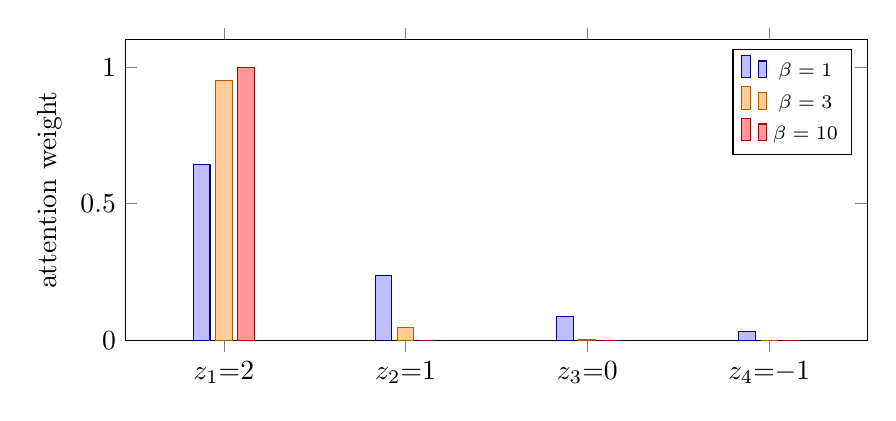
\begin{tikzpicture}
\begin{axis}[ybar,width=11cm,height=5.4cm,bar width=6pt,symbolic x coords={t1,t2,t3,t4},xtick=data,xticklabels={$z_1{=}2$,$z_2{=}1$,$z_3{=}0$,$z_4{=}{-}1$},
 ylabel={attention weight},ymin=0,ymax=1.1,enlarge x limits=0.18,legend style={font=\scriptsize,at={(0.98,0.97)},anchor=north east},nodes near coords style={font=\tiny}]
\addplot[fill=blue!25,draw=blue!60!black] coordinates {(t1,0.644) (t2,0.237) (t3,0.087) (t4,0.032)};
\addplot[fill=orange!40,draw=orange!70!black] coordinates {(t1,0.950) (t2,0.047) (t3,0.002) (t4,0.0)};
\addplot[fill=red!40,draw=red!70!black] coordinates {(t1,1.0) (t2,0.0) (t3,0.0) (t4,0.0)};
\legend{$\beta=1$,$\beta=3$,$\beta=10$}
\end{axis}
\end{tikzpicture}
\caption{$\softmax(\beta z)$ for $z=(2,1,0,-1)$ and growing $\beta$ (Proposition~\ref{prop:temp}): the soft distribution collapses onto the argmax.}
\end{figure}

\begin{intuition}
Softmax is a ``smooth argmax''. Large scores (or a large $\beta$) make it behave like the dictionary lookup; small scores make it an almost uniform average. Attention lives in between, and that is precisely what makes it \emph{differentiable}: a hard argmax is piecewise constant, so its gradient is $0$ almost everywhere and no learning signal can flow.
\end{intuition}

\subsection{Multi-head attention}\slides{24--25}
The SA layer can handle quasi-sparse dependencies (because of the softmax) and dynamic ones (because the attention function depends on the tokens). But what if a token depends on \emph{multiple subsets} of tokens (e.g.\ one for syntax, one for meaning)? The common generalization is \textbf{multi-head attention}.

\begin{definition}[Multi-head attention]
For $t=1,\dots,h$ compute separate queries, keys and values and a separate attention:
\[
Q_t=XW_{q,t},\quad K_t=XW_{k,t},\quad V_t=XW_{v,t},\qquad H_t=\softmax\!\Big(\frac{Q_tK_t^\top}{\sqrt q}\Big)V_t .
\]
The $h$ outputs are concatenated over the embedding dimension and re-projected with a trainable output matrix $W_o$:
\[
H=\big[\,H_1\;\|\;\cdots\;\|\;H_h\,\big]\,W_o .
\]
Hyper-parameters: embedding dimension $m$, output size $o$, number of heads $h$, and $q=v=m//h$ for all heads.
\end{definition}

\begin{proposition}[Parameter count]
With $q=v=m/h$ (integer division), $W_{q,t},W_{k,t},W_{v,t}\in\R^{d\times m/h}$ and $W_o\in\R^{m\times o}$, the layer has $3dm+mo$ parameters, \emph{independent of $h$}.
\end{proposition}
\begin{proof}
Each head has $3\cdot d\cdot\frac mh$ parameters; $h$ heads give $3dm$. The concatenation has width $h\cdot\frac mh=m$, so $W_o$ has $mo$ entries.
\end{proof}

\begin{example}
$d=m=o=512$ and $h=8$: each head works in dimension $q=v=64$ and the whole layer has $3\cdot512^2+512^2=4\cdot512^2\approx1.05\cdot10^6$ parameters, the same as a single head of width $512$. (The slide counts $3h$ trainable matrices, i.e.\ a $3\times h$ collection of $d\times q$ blocks.)
\end{example}

\begin{intuition}
Each head is a small, independent ``reader'' with its own notion of similarity, working in a smaller subspace ($64$ instead of $512$ dimensions). Splitting the width among heads costs nothing in parameters or FLOPs, but lets the layer attend to several different token subsets at once. $W_o$ finally mixes the heads' findings.
\end{intuition}

\subsection{Visualizing multi-head attention}\slides{26}
\begin{figure}[H]
\centering
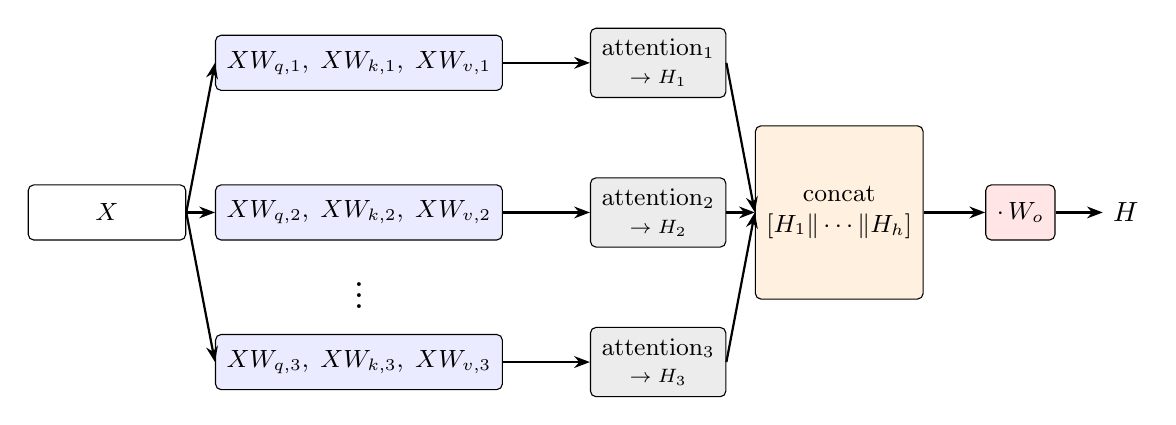
\begin{tikzpicture}
\node[box,minimum width=20mm] (X) at (0,0) {$X$};
\foreach \t/\y in {1/1.9,2/0.0,3/-1.9}{
 \node[box,fill=blue!8] (p\t) at (3.2,\y) {$XW_{q,\t},\;XW_{k,\t},\;XW_{v,\t}$};
 \node[box,fill=gray!15] (a\t) at (7.0,\y) {attention$_{\t}$\\[-1pt]{\scriptsize $\to H_{\t}$}};
 \draw[arr] (X.east) -- (p\t.west);
 \draw[arr] (p\t.east) -- (a\t.west);
}
\node[font=\Large] at (3.2,-0.95) {$\vdots$};
\node[box,minimum height=2.2cm,minimum width=14mm,fill=orange!12,align=center] (cat) at (9.3,0) {concat\\$[H_1\|\cdots\|H_h]$};
\foreach \t in {1,2,3}{\draw[arr] (a\t.east) -- (cat.west);}
\node[box,fill=red!10] (Wo) at (11.6,0) {$\cdot\,W_o$};
\draw[arr] (cat.east) -- (Wo.west);
\draw[arr] (Wo.east) -- ++(0.6,0) node[right] {$H$};
\end{tikzpicture}
\caption{Multi-head attention: $h$ independent projections and attentions, concatenation, output projection. Redrawn from slide 26 (adapted from D2L, Chapter 11.5).}
\end{figure}

%==========================================================
\section{The Transformer block}\slides{27--30}

\subsection{The transformer block}\slides{27}
In transformers the MHA layer is always used inside a more complex \textbf{transformer block}. The original block (Vaswani et al., 2017) is composed of an MHA layer, two layer normalizations, two residual connections and a position-wise network.

\begin{definition}[Layer normalization]
For a row $h\in\R^d$, $\LN(h)=\gamma\odot\dfrac{h-\mu(h)}{\sqrt{\sigma^2(h)+\varepsilon}}+\beta$, where $\mu,\sigma^2$ are the mean and variance of the $d$ entries of the row and $\gamma,\beta\in\R^d$ are trainable. Applied to a matrix, it acts on each row (token) independently.
\end{definition}

\begin{definition}[Transformer block (post-normalized)]\label{def:block}
Given $X\in\R^{n\times d}$:
\begin{enumerate}[nosep]
\item $H=\MHA(X)$;
\item $H=\LN(H+X)$ \hfill (residual + normalization);
\item $F=g(H)$, where the fully-connected model $g$ is applied on each row;
\item $H=\LN(F+H)$ \hfill (residual + normalization).
\end{enumerate}
\end{definition}

\subsection{Design of the block}\slides{28}
The design of the block is mostly based on \emph{empirical} considerations. Roughly, steps (1)--(2) are a \textbf{token mixing} operation (information flows between tokens), while steps (3)--(4) are a \textbf{per-token update}, akin to a $1\times1$ convolution. The block is similar in spirit to a \emph{depthwise separable convolution}. The intermediate MLP is typically a 2-layer MLP whose hidden dimension is an integer multiple of the input dimension (e.g.\ $3\times$, $4\times$), without biases.

\begin{proposition}[Parameters of a block]
Take $m=o=d$ in MHA and an MLP $d\to rd\to d$ without biases. Then (ignoring the LN parameters) the block has $4d^2+2rd^2=(4+2r)\,d^2$ parameters, i.e.\ $12d^2$ for $r=4$.
\end{proposition}
\begin{proof}
MHA has $3dm+mo=4d^2$ parameters (previous section); the MLP has $d\cdot rd+rd\cdot d=2rd^2$.
\end{proof}

\begin{example}
$d=512$, $r=4$: $12\cdot512^2\approx3.1\cdot10^6$ parameters per block. A stack of $12$ blocks has $\approx 3.8\cdot10^7$ parameters, plus embeddings.
\end{example}

\begin{intuition}
A block has two sub-steps that you can remember as ``\emph{talk, then think}'': first tokens talk to each other (attention mixes information \emph{across} tokens), then each token thinks on its own (the MLP transforms each row \emph{separately}, with the same weights). Residual connections let each block only add a correction to what it received.
\end{intuition}

\subsection{Pre- and post-normalized blocks}\slides{29}
\begin{figure}[H]
\centering
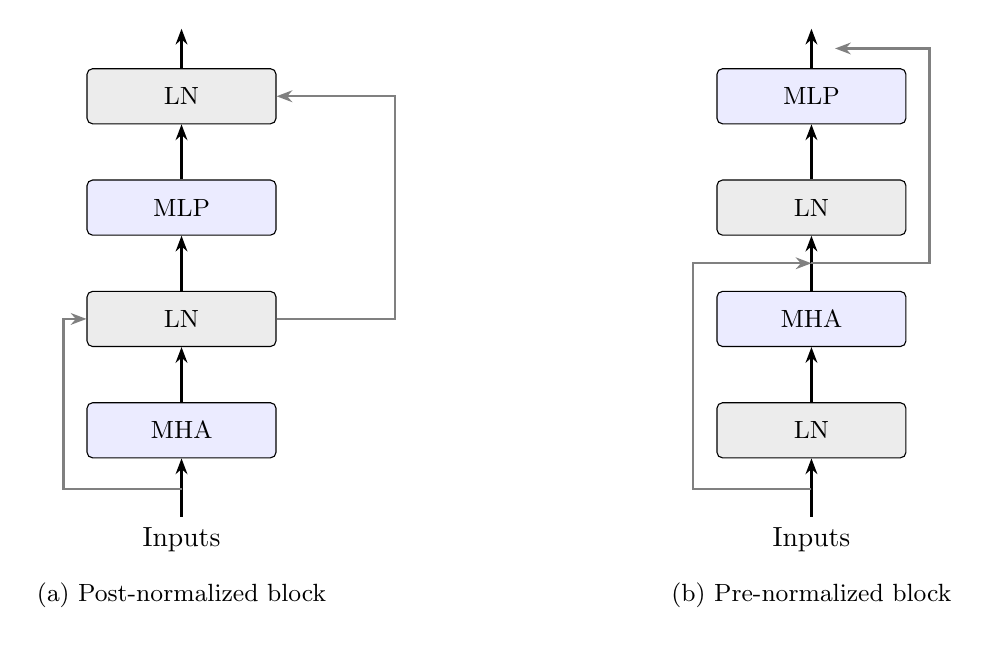
\begin{tikzpicture}[blk/.style={draw,rounded corners=2pt,minimum height=7mm,minimum width=24mm,inner sep=3pt,font=\small,align=center},node distance=7mm]
% (a) post
\begin{scope}
 \node[blk,fill=blue!8] (a1) at (0,0) {MHA};
 \node[blk,fill=gray!15,above=of a1] (a2) {LN};
 \node[blk,fill=blue!8,above=of a2] (a3) {MLP};
 \node[blk,fill=gray!15,above=of a3] (a4) {LN};
 \draw[arr] (0,-1.1) node[below]{Inputs} -- (a1.south);
 \draw[arr] (a1) -- (a2); \draw[arr] (a2) -- (a3); \draw[arr] (a3) -- (a4);
 \draw[arr] (a4.north) -- ++(0,0.5);
 \draw[arr,gray] (0,-0.75) -- ++(-1.5,0) |- (a2.west);
 \draw[arr,gray] (a2.east) ++(0,0) -- ++(1.5,0) |- (a4.east);
 \node[font=\small] at (0,-2.1) {(a) Post-normalized block};
\end{scope}
% (b) pre
\begin{scope}[xshift=8cm]
 \node[blk,fill=gray!15] (b1) at (0,0) {LN};
 \node[blk,fill=blue!8,above=of b1] (b2) {MHA};
 \node[blk,fill=gray!15,above=of b2] (b3) {LN};
 \node[blk,fill=blue!8,above=of b3] (b4) {MLP};
 \draw[arr] (0,-1.1) node[below]{Inputs} -- (b1.south);
 \draw[arr] (b1) -- (b2); \draw[arr] (b2) -- (b3); \draw[arr] (b3) -- (b4);
 \draw[arr] (b4.north) -- ++(0,0.5);
 \draw[arr,gray] (0,-0.75) -- ++(-1.5,0) |- ($(b2.north)!0.5!(b3.south)$);
 \draw[arr,gray] ($(b2.north)!0.5!(b3.south)$) -- ++(1.5,0) |- ($(b4.north)+(0.3,0.25)$);
 \node[font=\small] at (0,-2.1) {(b) Pre-normalized block};
\end{scope}
\end{tikzpicture}
\caption{Post-normalized (original) and pre-normalized blocks (redrawn from slide 29; gray lines are the residual connections, which are \emph{added} where they re-enter). The pre-normalized variant is usually simpler to train (Xiong et al., 2020).}
\end{figure}

\begin{definition}[Pre-normalized block]
$H=X+\MHA(\LN(X))$ and $Y=H+g(\LN(H))$.
\end{definition}

\begin{proposition}[Identity path in pre-norm stacks]
For a stack of pre-normalized blocks with $x_\ell=x_{\ell-1}+f_\ell(x_{\ell-1})$ (where $f_\ell$ collects the sub-layers of block $\ell$, including the LN inside), we have $x_L=x_0+\sum_{\ell=1}^{L}f_\ell(x_{\ell-1})$, so $\partial x_L/\partial x_0=I+\sum_\ell(\cdots)$ always contains an identity term.
\end{proposition}
\begin{proof}
Unroll the recursion by induction on $L$. The identity term in the Jacobian comes from the leading $x_0$.
\end{proof}

\begin{intuition}
In the post-norm block the signal must go through a normalization after \emph{every} residual sum, so there is no clean ``highway'' from input to output. In pre-norm the highway is untouched and the blocks only add their contributions to it, which is why very deep stacks train more easily.
\end{intuition}

\subsection{Variants of the transformer block}\slides{30}
Many other variants are now common, depending on the application and the computational constraints:
\begin{itemize}[nosep]
\item \textbf{Parallel variants} run MHA and MLP in parallel: $Y=X+\MHA(\LN X)+\mathrm{MLP}(\LN X)$ (the slide writes it compactly as $H=H+\mathrm{MLP}(H)+\MHA(H)$). The initial and final projections of the MLP and MHA can then be fused (Dehghani et al., 2023).
\item \textbf{Q/K-normalized variants} add additional LN operations on keys and queries (ibidem).
\item \textbf{Multi-query variants} share the same keys and values across the heads, to save computation (Shazeer, 2019).
\end{itemize}

\begin{proposition}[Key/value size under multi-query attention]
With $h$ heads of dimension $m/h$, standard MHA stores $2m$ numbers (keys and values) per token and per layer when decoding; sharing one $K,V$ pair across heads reduces this to $2m/h$, i.e.\ a factor $h$ smaller.
\end{proposition}
\begin{intuition}
The queries stay different per head (each reader asks its own question) but all readers consult the \emph{same} index card. This matters at generation time, when the keys/values of all previous tokens must be kept in memory (see the KV cache).
\end{intuition}

%==========================================================
\section{Positional embeddings}\slides{31--44}

\subsection{Permutation matrices}\slides{31}
\begin{definition}[Permutation matrix]
A permutation matrix $P\in\{0,1\}^{n\times n}$ has exactly one $1$ in every row and column. Left-multiplying a matrix $X$ by $P$ reorders its rows: $(PX)_i=X_{\pi(i)}$ for a permutation $\pi$ of $\{1,\dots,n\}$.
\end{definition}

\begin{example}
$P=\begin{psmallmatrix}1&0&0\\0&0&1\\0&1&0\end{psmallmatrix}$ gives $P\begin{psmallmatrix}x_1\\x_2\\x_3\end{psmallmatrix}=\begin{psmallmatrix}x_1\\x_3\\x_2\end{psmallmatrix}$.
\end{example}

\begin{lemma}\label{lem:perm}
$P^\top P=PP^\top=I$.
\end{lemma}
\begin{proof}
$(P^\top P)_{ij}=\sum_l P_{li}P_{lj}$ is $1$ iff the unique $1$ in column $i$ and the unique $1$ in column $j$ are in the same row, i.e.\ iff $i=j$.
\end{proof}

\subsection{The MHA layer is equivariant to permutations}\slides{32}
In audio and text the $i$-th row of $X$ is a single time step or a single token (e.g.\ a word). In an MHA layer the ordering is lost because the layer is \emph{equivariant} to it (similar to the GAT layer for graphs).

\begin{definition}[Permutation equivariance]
A function $f$ is equivariant to permutations if $f(PX)=P\,f(X)$ for every permutation matrix $P$.
\end{definition}

\begin{lemma}[Row-wise softmax commutes with permutations]\label{lem:sm-perm}
For any square matrix $A$ and permutation matrix $P$: $\softmax(PAP^\top)=P\,\softmax(A)\,P^\top$.
\end{lemma}
\begin{proof}
With $(PX)_i=X_{\pi(i)}$ we have $(PAP^\top)_{ij}=A_{\pi(i)\pi(j)}$. The normalizer of row $i$ is $\sum_j e^{A_{\pi(i)\pi(j)}}=\sum_l e^{A_{\pi(i)l}}$ (re-index $l=\pi(j)$), the normalizer of row $\pi(i)$ of $A$. Hence $\softmax(PAP^\top)_{ij}=\softmax(A)_{\pi(i)\pi(j)}=(P\softmax(A)P^\top)_{ij}$.
\end{proof}

\begin{theorem}[MHA is permutation equivariant]\label{thm:equiv}
For every permutation matrix $P$, $\MHA(PX)=P\cdot\MHA(X)$.
\end{theorem}
\begin{proof}
For one head, $Q'=PXW_q=PQ$, $K'=PK$, $V'=PV$. By Lemmas~\ref{lem:sm-perm} and~\ref{lem:perm},
\[
\softmax\!\Big(\tfrac{PQK^\top P^\top}{\sqrt q}\Big)PV=P\,\softmax\!\Big(\tfrac{QK^\top}{\sqrt q}\Big)P^\top P\,V=P\,H_t .
\]
Concatenation over heads and right-multiplication by $W_o$ act on columns, so they commute with the row permutation $P$.
\end{proof}

\begin{corollary}\label{cor:bag}
The whole transformer block (the LN and the MLP act row by row, residuals preserve equivariance) and any stack of blocks are permutation equivariant. If the output is pooled over tokens (e.g.\ global average pooling), the model is permutation \emph{invariant}: it sees a ``bag of tokens''.
\end{corollary}

\begin{example}
In Example~\ref{ex:toy}, swapping tokens $x_1$ and $x_2$ simply swaps the first two output rows: $(0.60,0.80),(0.80,0.60),(0.75,0.75)$. For text, ``dog bites man'' and ``man bites dog'' would be processed identically up to a reordering of the rows, so mean-pooled outputs would be \emph{equal}.
\end{example}

\begin{intuition}
Attention treats the input as a \emph{set}: it only asks ``which tokens are similar to me?'', never ``where am I?''. A convolution knows positions implicitly (its kernel has a left and a right), attention does not. This is not a good property for sequences, so we must give the model the position explicitly.
\end{intuition}

\subsection{Visualizing permutation equivariance}\slides{33}
\begin{figure}[H]
\centering
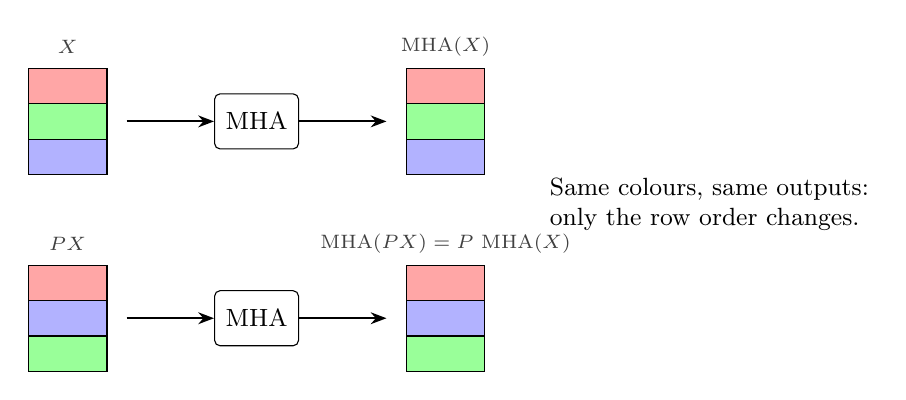
\begin{tikzpicture}[r/.style={minimum width=10mm,minimum height=4.5mm,draw,inner sep=0}]
% top row
\foreach \c/\y in {red!35/0.9,green!40/0.45,blue!30/0}{\node[r,fill=\c] at (0,\y) {};}
\node[box] (m1) at (2.4,0.45) {MHA};
\foreach \c/\y in {red!35/0.9,green!40/0.45,blue!30/0}{\node[r,fill=\c] at (4.8,\y) {};}
\draw[arr] (0.75,0.45) -- (m1.west); \draw[arr] (m1.east) -- (4.05,0.45);
\node[lbl] at (0,1.4) {$X$}; \node[lbl] at (4.8,1.4) {$\MHA(X)$};
% bottom row
\foreach \c/\y in {red!35/-1.6,blue!30/-2.05,green!40/-2.5}{\node[r,fill=\c] at (0,\y) {};}
\node[box] (m2) at (2.4,-2.05) {MHA};
\foreach \c/\y in {red!35/-1.6,blue!30/-2.05,green!40/-2.5}{\node[r,fill=\c] at (4.8,\y) {};}
\draw[arr] (0.75,-2.05) -- (m2.west); \draw[arr] (m2.east) -- (4.05,-2.05);
\node[lbl] at (0,-1.1) {$PX$}; \node[lbl] at (4.8,-1.1) {$\MHA(PX)=P\,\MHA(X)$};
\node[font=\small,align=left,anchor=west] at (6.0,-0.6) {Same colours, same outputs:\\only the row order changes.};
\end{tikzpicture}
\caption{Permuting the rows of the input permutes the rows of the output in the same way. Redrawn from slide 33.}
\end{figure}

\subsection{Positional embeddings}\slides{34}
\begin{definition}[Positional embeddings]
Before the first MHA layer we concatenate or sum to the input a matrix $E\in\R^{n\times e}$ of positional embeddings,
\[
X'=[X\,\|\,E]\qquad\text{or}\qquad X'=X+E\ (e=d),
\]
where each row $[E]_i$ should uniquely encode the position of the $i$-th element of the sequence.
\end{definition}
This breaks equivariance: in general $\MHA(PX\,\|\,E)\neq P\cdot\MHA(X\,\|\,E)$.

\begin{example}[Equivariance is lost]\label{ex:posbreak}
Take $d=2$, identity projections, $X=\begin{psmallmatrix}1&0\\0&1\end{psmallmatrix}$, $E=\begin{psmallmatrix}0&0\\1&1\end{psmallmatrix}$, $P$ the swap. Then
$\MHA(X+E)\approx\begin{psmallmatrix}1&1\\1&1.89\end{psmallmatrix}$, so $P\,\MHA(X+E)\approx\begin{psmallmatrix}1&1.89\\1&1\end{psmallmatrix}$, but
$\MHA(PX+E)\approx\begin{psmallmatrix}1&1\\1.89&1\end{psmallmatrix}$. The two differ: the model is now sensitive to \emph{where} each token sits.
\end{example}

\subsection{Visualization of positional embeddings}\slides{35}
\begin{figure}[H]
\centering
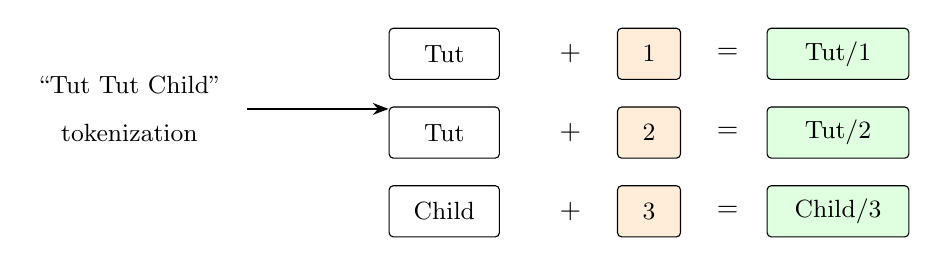
\begin{tikzpicture}
\node[font=\small] at (-1.0,0.6) {``Tut Tut Child''};
\node[font=\small] at (-1.0,0.0) {tokenization};
\foreach \w/\p/\y in {Tut/1/1.0,Tut/2/0.0,Child/3/-1.0}{
 \node[tok,minimum width=14mm] (w\p) at (3,\y) {\w};
 \node at (4.6,\y) {$+$};
 \node[tok,fill=orange!15,minimum width=8mm] (p\p) at (5.6,\y) {\p};
 \node at (6.6,\y) {$=$};
 \node[tok,fill=green!12,minimum width=18mm] (o\p) at (8.0,\y) {\w/\p};
}
\draw[arr] (0.5,0.3) -- (w2.west |- 0.3,0.3);
\end{tikzpicture}
\caption{The same token at two different positions is now represented by different vectors after adding the positional embeddings (here shown symbolically as ``token/position''). Redrawn from slide 35.}
\end{figure}

\subsection{Simple positional embeddings}\slides{36}
For a sequence of maximum length $p$ we can encode the position with a one-hot vector of dimension $p$,
\[
E_0=[1,0,0,\dots],\quad E_1=[0,1,0,\dots],\quad E_2=[0,0,1,\dots],\ \dots
\]
or with a single increasing scalar,
\[
E_0=[0/p],\quad E_1=[1/p],\quad E_2=[2/p],\ \dots
\]
Both strategies are not particularly good empirically.

\begin{intuition}
One-hot positions say ``you are at slot 7'' but, as with one-hot words, every pair of positions is equally far apart ($\sqrt2$), so neighbouring positions are not recognized as neighbours. The scalar version has the opposite problem: a single number in $[0,1)$ is a very weak and badly scaled signal compared to $d$-dimensional token embeddings.
\end{intuition}

\subsection{Trainable positional embeddings}\slides{37}
We can \emph{learn} the positional embeddings with an embedding layer (e.g.\ \texttt{tf.keras.layers.Embedding}): to each position $i$ we associate an embedding vector of fixed dimension, trained with the rest of the network. We need to fix the \textbf{maximum length} of the sentence; for longer ones, the set of vectors is \emph{linearly interpolated} up to a larger size (the strategy used in BERT and in the Vision Transformer described below).

\subsection{Sinusoidal embeddings}\slides{38}
Consider a single sinusoidal function of frequency $\omega$: $[E]_i=\sin(i\omega)$. Interpret it as a \textbf{clock} with frequency $\omega$: for two points inside a single rotation it gives their relative distance; for other points, the distance is only precise modulo the period.

\subsection{Multiple sinusoidal embeddings}\slides{39}
To uniquely identify any possible position we use multiple sinusoids, each with a frequency $\omega_j$, $j=1,\dots,e$:
\[
E_i=[\sin(i\omega_0),\sin(i\omega_1),\dots,\sin(i\omega_e)].
\]
Think of a clock with $e$ different hands, each rotating at its own frequency. This representation can generalize to any length, with no maximum length imposed a priori.

\subsection{Choosing the frequency}\slides{40}
An empirically good choice (popularized by Vaswani et al., 2017) is
\[
\omega_j=\frac1{10000^{\,j/e}} .
\]
For $j=0$ the period is $2\pi$; for $j=e$ it is $10000\cdot2\pi$; in between, the periods increase in a \emph{geometric progression}. To reduce parameters it is common to \emph{sum} the encodings instead of concatenating them ($e=d$): $X'=X+E$.

\begin{table}[ht]
\centering\small
\begin{tabular}{@{}c|ccccccccc@{}}
\toprule
$j$ & 0&1&2&3&4&5&6&7&8\\
\midrule
period $2\pi\cdot10000^{j/8}$ & 6.3 & 19.9 & 62.8 & 199 & 628 & 1987 & 6283 & 19869 & 62832\\
\bottomrule
\end{tabular}
\caption{Periods of the $e=8$ clock hands: each hand is $\sqrt{10}\approx3.16$ times slower than the previous one.}
\end{table}

\begin{intuition}
It works like a clock showing seconds, minutes and hours at once (but with ratios of $\approx3.16$ instead of $60$). The fastest hand tells you the position \emph{precisely} within a short range, the slower hands tell you \emph{roughly where in the long range}. Together they identify a position, up to very large lengths, with no table to learn.
\end{intuition}

\subsection{Final version}\slides{41}
A popular extension alternates sines and cosines of the same frequency:
\begin{align}
[E]_{i,2j}&=\sin\!\Big(\frac{i}{10000^{2j/e}}\Big),\label{eq:pe-sin}\\
[E]_{i,2j+1}&=\cos\!\Big(\frac{i}{10000^{2j/e}}\Big).\label{eq:pe-cos}
\end{align}

\begin{proposition}[Shift = rotation]\label{prop:shift}
For each offset $p$ there is a matrix $T(p)$ such that $[E]_{i+p}=[E]_i\,T(p)$ for all $i$. $T(p)$ is block diagonal with $2\times2$ rotation blocks $\begin{psmallmatrix}\cos p\omega_j&-\sin p\omega_j\\\sin p\omega_j&\cos p\omega_j\end{psmallmatrix}$, $\omega_j=10000^{-2j/e}$.
\end{proposition}
\begin{proof}
For the $j$-th pair, with row vector $(\sin i\omega,\cos i\omega)$, the angle-addition formulas give
$\sin((i{+}p)\omega)=\sin i\omega\cos p\omega+\cos i\omega\sin p\omega$ and $\cos((i{+}p)\omega)=-\sin i\omega\sin p\omega+\cos i\omega\cos p\omega$, which is exactly $(\sin i\omega,\cos i\omega)\begin{psmallmatrix}\cos p\omega&-\sin p\omega\\\sin p\omega&\cos p\omega\end{psmallmatrix}$. $T(p)$ does not depend on $i$.
\end{proof}

\begin{corollary}[Dot products see only the offset]
$[E]_i\,[E]_{i+p}^\top=\sum_{j}\cos(p\,\omega_j)$, which does not depend on $i$. In particular all rows have the same norm $\sqrt{e/2}$.
\end{corollary}
\begin{proof}
For each pair, $\sin a\sin b+\cos a\cos b=\cos(a-b)$ with $a=i\omega_j$, $b=(i{+}p)\omega_j$. For $p=0$ every term is $1$ and there are $e/2$ pairs.
\end{proof}

\begin{intuition}
Adding $p$ to the position just \emph{rotates} every clock hand by a fixed amount. A network can therefore learn ``look $p$ steps back'' as a single linear operation, no matter what the absolute position is.
\end{intuition}

\subsection{Visualizing positional encodings}\slides{42}
\begin{figure}[H]
\centering
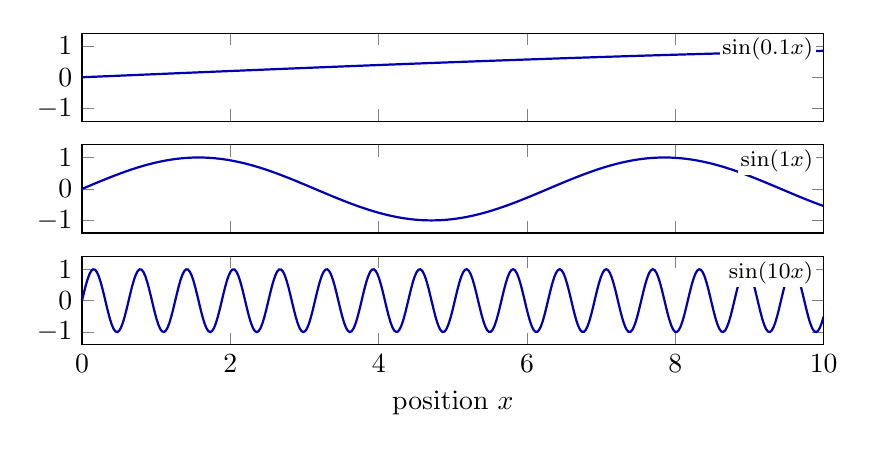
\begin{tikzpicture}
\begin{groupplot}[group style={group size=1 by 3,vertical sep=3mm,x descriptions at=edge bottom},width=11cm,height=2.7cm,xmin=0,xmax=10,ymin=-1.4,ymax=1.4,ytick={-1,0,1},xtick={0,2,4,6,8,10},samples=400,domain=0:10]
\nextgroupplot\addplot[thick,blue!70!black]{sin(deg(0.1*x))};\node[anchor=north east,font=\footnotesize,fill=white,inner sep=1pt] at (rel axis cs:0.99,0.98) {$\sin(0.1x)$};
\nextgroupplot\addplot[thick,blue!70!black]{sin(deg(x))};\node[anchor=north east,font=\footnotesize,fill=white,inner sep=1pt] at (rel axis cs:0.99,0.98) {$\sin(1x)$};
\nextgroupplot[xlabel={position $x$}]\addplot[thick,blue!70!black]{sin(deg(10*x))};\node[anchor=north east,font=\footnotesize,fill=white,inner sep=1pt] at (rel axis cs:0.99,0.98) {$\sin(10x)$};
\end{groupplot}
\end{tikzpicture}
\caption{Sinusoids of different frequencies (as in slide 42, from book Chapter 10.6). A slow one varies little across the whole range; a fast one distinguishes close positions.}
\end{figure}

\begin{figure}[H]
\centering
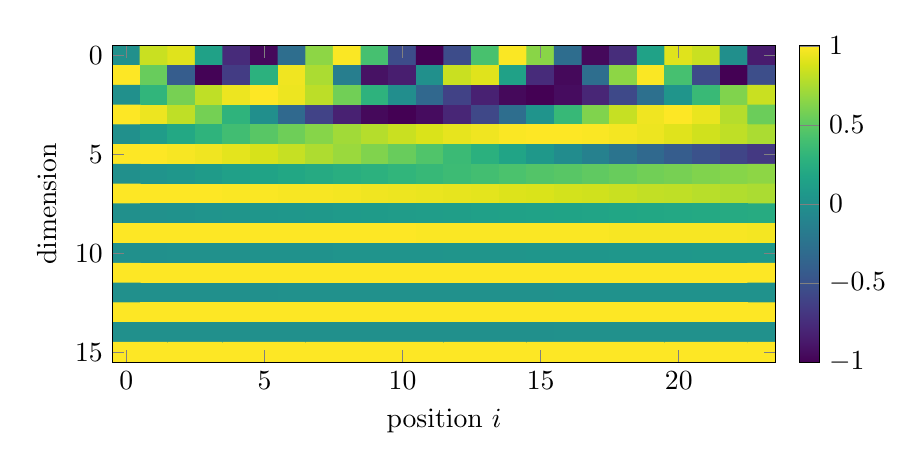
\begin{tikzpicture}
\begin{axis}[width=10cm,height=5.6cm,colormap/viridis,colorbar,colorbar style={width=2.5mm},xlabel={position $i$},ylabel={dimension},point meta min=-1,point meta max=1,
 y dir=reverse,enlargelimits=false,axis on top,ytick={0,5,10,15}]
\addplot[matrix plot*,point meta=explicit,mesh/cols=24,mesh/rows=16] table[row sep=\\,meta index=2] {
x y v\\
0 0 0.00\\
1 0 0.84\\
2 0 0.91\\
3 0 0.14\\
4 0 -0.76\\
5 0 -0.96\\
6 0 -0.28\\
7 0 0.66\\
8 0 0.99\\
9 0 0.41\\
10 0 -0.54\\
11 0 -1.00\\
12 0 -0.54\\
13 0 0.42\\
14 0 0.99\\
15 0 0.65\\
16 0 -0.29\\
17 0 -0.96\\
18 0 -0.75\\
19 0 0.15\\
20 0 0.91\\
21 0 0.84\\
22 0 -0.01\\
23 0 -0.85\\
0 1 1.00\\
1 1 0.54\\
2 1 -0.42\\
3 1 -0.99\\
4 1 -0.65\\
5 1 0.28\\
6 1 0.96\\
7 1 0.75\\
8 1 -0.15\\
9 1 -0.91\\
10 1 -0.84\\
11 1 0.00\\
12 1 0.84\\
13 1 0.91\\
14 1 0.14\\
15 1 -0.76\\
16 1 -0.96\\
17 1 -0.28\\
18 1 0.66\\
19 1 0.99\\
20 1 0.41\\
21 1 -0.55\\
22 1 -1.00\\
23 1 -0.53\\
0 2 0.00\\
1 2 0.31\\
2 2 0.59\\
3 2 0.81\\
4 2 0.95\\
5 2 1.00\\
6 2 0.95\\
7 2 0.80\\
8 2 0.57\\
9 2 0.29\\
10 2 -0.02\\
11 2 -0.33\\
12 2 -0.61\\
13 2 -0.82\\
14 2 -0.96\\
15 2 -1.00\\
16 2 -0.94\\
17 2 -0.79\\
18 2 -0.56\\
19 2 -0.27\\
20 2 0.04\\
21 2 0.35\\
22 2 0.62\\
23 2 0.84\\
0 3 1.00\\
1 3 0.95\\
2 3 0.81\\
3 3 0.58\\
4 3 0.30\\
5 3 -0.01\\
6 3 -0.32\\
7 3 -0.60\\
8 3 -0.82\\
9 3 -0.96\\
10 3 -1.00\\
11 3 -0.94\\
12 3 -0.79\\
13 3 -0.57\\
14 3 -0.28\\
15 3 0.03\\
16 3 0.34\\
17 3 0.62\\
18 3 0.83\\
19 3 0.96\\
20 3 1.00\\
21 3 0.94\\
22 3 0.78\\
23 3 0.55\\
0 4 0.00\\
1 4 0.10\\
2 4 0.20\\
3 4 0.30\\
4 4 0.39\\
5 4 0.48\\
6 4 0.56\\
7 4 0.64\\
8 4 0.72\\
9 4 0.78\\
10 4 0.84\\
11 4 0.89\\
12 4 0.93\\
13 4 0.96\\
14 4 0.99\\
15 4 1.00\\
16 4 1.00\\
17 4 0.99\\
18 4 0.97\\
19 4 0.95\\
20 4 0.91\\
21 4 0.86\\
22 4 0.81\\
23 4 0.75\\
0 5 1.00\\
1 5 1.00\\
2 5 0.98\\
3 5 0.96\\
4 5 0.92\\
5 5 0.88\\
6 5 0.83\\
7 5 0.76\\
8 5 0.70\\
9 5 0.62\\
10 5 0.54\\
11 5 0.45\\
12 5 0.36\\
13 5 0.27\\
14 5 0.17\\
15 5 0.07\\
16 5 -0.03\\
17 5 -0.13\\
18 5 -0.23\\
19 5 -0.32\\
20 5 -0.42\\
21 5 -0.50\\
22 5 -0.59\\
23 5 -0.67\\
0 6 0.00\\
1 6 0.03\\
2 6 0.06\\
3 6 0.09\\
4 6 0.13\\
5 6 0.16\\
6 6 0.19\\
7 6 0.22\\
8 6 0.25\\
9 6 0.28\\
10 6 0.31\\
11 6 0.34\\
12 6 0.37\\
13 6 0.40\\
14 6 0.43\\
15 6 0.46\\
16 6 0.48\\
17 6 0.51\\
18 6 0.54\\
19 6 0.57\\
20 6 0.59\\
21 6 0.62\\
22 6 0.64\\
23 6 0.66\\
0 7 1.00\\
1 7 1.00\\
2 7 1.00\\
3 7 1.00\\
4 7 0.99\\
5 7 0.99\\
6 7 0.98\\
7 7 0.98\\
8 7 0.97\\
9 7 0.96\\
10 7 0.95\\
11 7 0.94\\
12 7 0.93\\
13 7 0.92\\
14 7 0.90\\
15 7 0.89\\
16 7 0.87\\
17 7 0.86\\
18 7 0.84\\
19 7 0.82\\
20 7 0.81\\
21 7 0.79\\
22 7 0.77\\
23 7 0.75\\
0 8 0.00\\
1 8 0.01\\
2 8 0.02\\
3 8 0.03\\
4 8 0.04\\
5 8 0.05\\
6 8 0.06\\
7 8 0.07\\
8 8 0.08\\
9 8 0.09\\
10 8 0.10\\
11 8 0.11\\
12 8 0.12\\
13 8 0.13\\
14 8 0.14\\
15 8 0.15\\
16 8 0.16\\
17 8 0.17\\
18 8 0.18\\
19 8 0.19\\
20 8 0.20\\
21 8 0.21\\
22 8 0.22\\
23 8 0.23\\
0 9 1.00\\
1 9 1.00\\
2 9 1.00\\
3 9 1.00\\
4 9 1.00\\
5 9 1.00\\
6 9 1.00\\
7 9 1.00\\
8 9 1.00\\
9 9 1.00\\
10 9 1.00\\
11 9 0.99\\
12 9 0.99\\
13 9 0.99\\
14 9 0.99\\
15 9 0.99\\
16 9 0.99\\
17 9 0.99\\
18 9 0.98\\
19 9 0.98\\
20 9 0.98\\
21 9 0.98\\
22 9 0.98\\
23 9 0.97\\
0 10 0.00\\
1 10 0.00\\
2 10 0.01\\
3 10 0.01\\
4 10 0.01\\
5 10 0.02\\
6 10 0.02\\
7 10 0.02\\
8 10 0.03\\
9 10 0.03\\
10 10 0.03\\
11 10 0.03\\
12 10 0.04\\
13 10 0.04\\
14 10 0.04\\
15 10 0.05\\
16 10 0.05\\
17 10 0.05\\
18 10 0.06\\
19 10 0.06\\
20 10 0.06\\
21 10 0.07\\
22 10 0.07\\
23 10 0.07\\
0 11 1.00\\
1 11 1.00\\
2 11 1.00\\
3 11 1.00\\
4 11 1.00\\
5 11 1.00\\
6 11 1.00\\
7 11 1.00\\
8 11 1.00\\
9 11 1.00\\
10 11 1.00\\
11 11 1.00\\
12 11 1.00\\
13 11 1.00\\
14 11 1.00\\
15 11 1.00\\
16 11 1.00\\
17 11 1.00\\
18 11 1.00\\
19 11 1.00\\
20 11 1.00\\
21 11 1.00\\
22 11 1.00\\
23 11 1.00\\
0 12 0.00\\
1 12 0.00\\
2 12 0.00\\
3 12 0.00\\
4 12 0.00\\
5 12 0.00\\
6 12 0.01\\
7 12 0.01\\
8 12 0.01\\
9 12 0.01\\
10 12 0.01\\
11 12 0.01\\
12 12 0.01\\
13 12 0.01\\
14 12 0.01\\
15 12 0.01\\
16 12 0.02\\
17 12 0.02\\
18 12 0.02\\
19 12 0.02\\
20 12 0.02\\
21 12 0.02\\
22 12 0.02\\
23 12 0.02\\
0 13 1.00\\
1 13 1.00\\
2 13 1.00\\
3 13 1.00\\
4 13 1.00\\
5 13 1.00\\
6 13 1.00\\
7 13 1.00\\
8 13 1.00\\
9 13 1.00\\
10 13 1.00\\
11 13 1.00\\
12 13 1.00\\
13 13 1.00\\
14 13 1.00\\
15 13 1.00\\
16 13 1.00\\
17 13 1.00\\
18 13 1.00\\
19 13 1.00\\
20 13 1.00\\
21 13 1.00\\
22 13 1.00\\
23 13 1.00\\
0 14 0.00\\
1 14 0.00\\
2 14 0.00\\
3 14 0.00\\
4 14 0.00\\
5 14 0.00\\
6 14 0.00\\
7 14 0.00\\
8 14 0.00\\
9 14 0.00\\
10 14 0.00\\
11 14 0.00\\
12 14 0.00\\
13 14 0.00\\
14 14 0.00\\
15 14 0.00\\
16 14 0.01\\
17 14 0.01\\
18 14 0.01\\
19 14 0.01\\
20 14 0.01\\
21 14 0.01\\
22 14 0.01\\
23 14 0.01\\
0 15 1.00\\
1 15 1.00\\
2 15 1.00\\
3 15 1.00\\
4 15 1.00\\
5 15 1.00\\
6 15 1.00\\
7 15 1.00\\
8 15 1.00\\
9 15 1.00\\
10 15 1.00\\
11 15 1.00\\
12 15 1.00\\
13 15 1.00\\
14 15 1.00\\
15 15 1.00\\
16 15 1.00\\
17 15 1.00\\
18 15 1.00\\
19 15 1.00\\
20 15 1.00\\
21 15 1.00\\
22 15 1.00\\
23 15 1.00\\
};
\end{axis}
\end{tikzpicture}
\caption{Original figure: the matrix $E$ of Eqs.~\eqref{eq:pe-sin}--\eqref{eq:pe-cos} for $24$ positions and $e=16$ (even rows are sines, odd rows cosines). The first dimensions oscillate fast with the position, the last ones almost not at all.}
\end{figure}

\subsection{Relative positional embeddings}\slides{43}
Another possibility is \emph{relative} positional embeddings: the attention function is modified to depend on the relative distance $i-j$ between tokens.

\begin{definition}[Attention with linear biases (ALiBi)]
\begin{equation}\label{eq:alibi}
\alpha(x_i,x_j,i-j)=x_i^\top x_j+b_{ij},
\end{equation}
where $b_{ij}=b(i-j)$ is a bias depending on the offset (trainable, in the slide's formulation; in the original ALiBi paper it is $-m_h|i-j|$ with a fixed slope $m_h$ per head: Press et al., 2021).
\end{definition}

Another common option is \textbf{rotary position embeddings (RoPE)} (Su et al., 2021).

\begin{proposition}[Rotary embeddings are relative]
Let $R_\theta$ be the $2\times2$ rotation by angle $\theta$ and rotate the 2D query at position $i$ by $i\theta$ and the key at position $j$ by $j\theta$. Then $(R_{i\theta}q)^\top(R_{j\theta}k)=q^\top R_{(j-i)\theta}\,k$ depends on positions only through $j-i$. (In practice the $d$ dimensions are split into 2D pairs, each with its own $\theta$.)
\end{proposition}
\begin{proof}
$R_a^\top=R_{-a}$ and $R_{-a}R_b=R_{b-a}$.
\end{proof}

\begin{intuition}
Absolute positions answer ``which seat am I in?''. Relative schemes answer ``how far is that token from me?'', which is usually what matters for language (a verb cares about its subject being 3 words back, not about the absolute index). ALiBi simply \emph{penalizes} far-away tokens linearly; RoPE rotates queries and keys so that only the angle difference survives in their dot product.
\end{intuition}

\subsection{Visualization of ALiBi}\slides{44}
\begin{figure}[H]
\centering
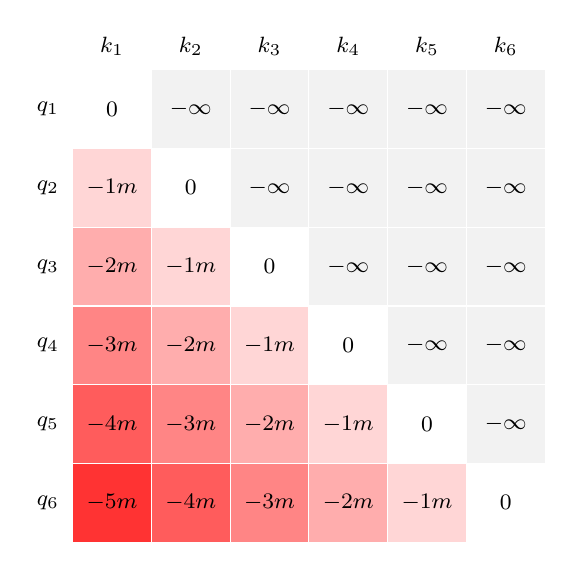
\begin{tikzpicture}[cell/.style={minimum size=10mm,inner sep=0,font=\footnotesize}]
\foreach \i in {1,...,6}{
 \foreach \j in {1,...,6}{
  \ifnum\j>\i
    \node[cell,fill=gray!10,draw=white] at (\j,-\i) {$-\infty$};
  \else
    \pgfmathtruncatemacro{\d}{\i-\j}
    \pgfmathtruncatemacro{\pc}{\d*16}
    \node[cell,fill=red!\pc!white,draw=white] at (\j,-\i) {\ifnum\d=0 $0$\else $-\d m$\fi};
  \fi
 }}
\foreach \i in {1,...,6}{\node[font=\footnotesize] at (\i,-0.2) {$k_\i$}; \node[font=\footnotesize,anchor=east] at (0.45,-\i) {$q_\i$};}
\end{tikzpicture}
\caption{Bias matrix added to the scores $q_i^\top k_j$ in a causal ALiBi model: the penalty grows linearly with the distance $i-j$ (slope $m$), with no learned position vectors. Original TikZ redrawing of the idea shown on slide 44 (reproduced there from Press et al., 2021).}
\end{figure}

\begin{intuition}
The further back a token is, the more its score is reduced before the softmax, so by default tokens pay more attention to their neighbours. Since the rule is a formula (not a table), the model can be tested on sequences longer than those seen in training (``train short, test long'').
\end{intuition}

%==========================================================
\section{The complete transformer model}\slides{45--46}

\subsection{Putting everything together}\slides{45}
\begin{definition}[Transformer (encoder-only)]
Given a tokenized and embedded sequence $X\in\R^{n\times d}$ and positional embeddings $E$:
\[
X_0=X+E,\qquad X_\ell=\mathrm{Block}_\ell(X_{\ell-1}),\ \ \ell=1,\dots,L .
\]
The final model is built with positional encodings and a \emph{stack} of blocks (called $n$ in the slide's figure; here $L$, to avoid a clash with the sequence length).
\end{definition}

\begin{figure}[H]
\centering
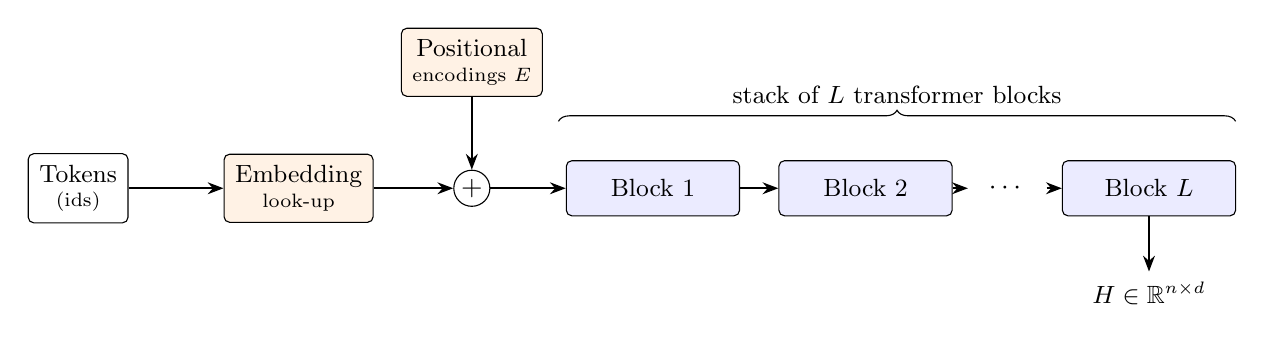
\begin{tikzpicture}
\node[box] (tok) at (0,0) {Tokens\\[-2pt]{\scriptsize (ids)}};
\node[box,fill=orange!10] (emb) at (2.8,0) {Embedding\\[-2pt]{\scriptsize look-up}};
\node[draw,circle,inner sep=1pt] (plus) at (5.0,0) {$+$};
\node[box,fill=orange!10] (pos) at (5.0,1.6) {Positional\\[-2pt]{\scriptsize encodings $E$}};
\node[box,fill=blue!8,minimum width=22mm] (b1) at (7.3,0) {Block 1};
\node[box,fill=blue!8,minimum width=22mm] (b2) at (10.0,0) {Block 2};
\node at (11.8,0) {$\cdots$};
\node[box,fill=blue!8,minimum width=22mm] (bn) at (13.6,0) {Block $L$};
\draw[arr] (tok)--(emb); \draw[arr] (emb)--(plus); \draw[arr] (pos)--(plus);
\draw[arr] (plus)--(b1); \draw[arr] (b1)--(b2); \draw[arr] (b2)--(11.3,0); \draw[arr] (12.3,0)--(bn);
\draw[arr] (bn.south) -- ++(0,-0.7) node[below,font=\small] {$H\in\R^{n\times d}$};
\draw[decorate,decoration={brace,amplitude=4pt}] (6.1,0.85) -- (14.7,0.85) node[midway,above=3pt,font=\small] {stack of $L$ transformer blocks};
\end{tikzpicture}
\caption{The complete (encoder-only) transformer. Redrawn from slide 45 (adapted from Chapter 10.7 of the book).}
\end{figure}

\subsection{Classification token}\slides{46}
To perform classification or regression we can apply a final global pooling over the $n$ tokens and one or more fully-connected layers. An alternative that works well empirically is the \textbf{class token}.

\begin{definition}[Class token]
Add an extra trainable token $c\in\R^d$ to the input matrix,
\[
X'=\begin{bmatrix}X\\ c^\top\end{bmatrix}\in\R^{(n+1)\times d},
\]
apply the transformer, $H=\mathrm{Transformer}(X')$, and classify from its last row:
\[
y=\softmax\!\big(W^\top[H]_{n+1}\big).
\]
\end{definition}

\begin{intuition}
The class token is an empty notepad appended to the sequence. It has no content of its own, but at every layer it can \emph{attend to all the real tokens} and write down a summary; after $L$ blocks its row is a learned, task-specific pooling of the whole input. It costs only $d$ extra parameters and adds one row to the $n\times n$ attention matrix.
\end{intuition}

%==========================================================
\section{Causal models and encoder-decoder models}\slides{47--55}

\subsection{Encoder-decoder models}\slides{47}
The original transformer was a more general model for \textbf{sequence-to-sequence (seq2seq)} tasks such as machine translation (a variable number of tokens in input and in output). It \emph{encoded} the input sequence, which was then \emph{decoded} by a second, masked transformer that generated the output sequence. To understand it we need three further mechanisms: \textbf{autoregression}, \textbf{masked attention} and \textbf{cross-attention}. The model described so far is sometimes called an \emph{encoder-only} transformer.

\subsection{Autoregressive models}\slides{48}
Autoregressive models generate data (here: tokens) one by one, feeding the predicted values back to the input: we prompt the model with the beginning of the sequence and let it forecast the next step; we concatenate it to the input and prompt again, and so on.

During training we can feed the network only true samples (\textbf{teacher forcing}) or mix in some of the network's own predictions. Extrapolating outside the training windows may still be difficult.

\begin{proposition}[Chain rule factorization]\label{prop:chain}
Any joint distribution over a sequence factorizes exactly as $p(x_1,\dots,x_n)=\prod_{t=1}^{n}p(x_t\mid x_1,\dots,x_{t-1})$. An autoregressive model parameterizes the conditionals and so models the joint exactly, without further independence assumptions.
\end{proposition}
\begin{proof}
Repeated application of $p(a,b)=p(a)\,p(b\mid a)$.
\end{proof}

\subsection{An example}\slides{49}
Suppose $n=4$ and we have observed two values $x_1,x_2$. We call the model a first time on the sequence padded with zeros; position $2$ of the output is the forecast $\hat x_3$ (the model's outputs at other positions are not used, ``$-$''). We add $\hat x_3$ to the sequence and call the model again, now obtaining $\hat x_4$, and so on (the predicted values are in color in the slide); when the window of length $4$ is full, the oldest values slide out.

\begin{figure}[H]
\centering
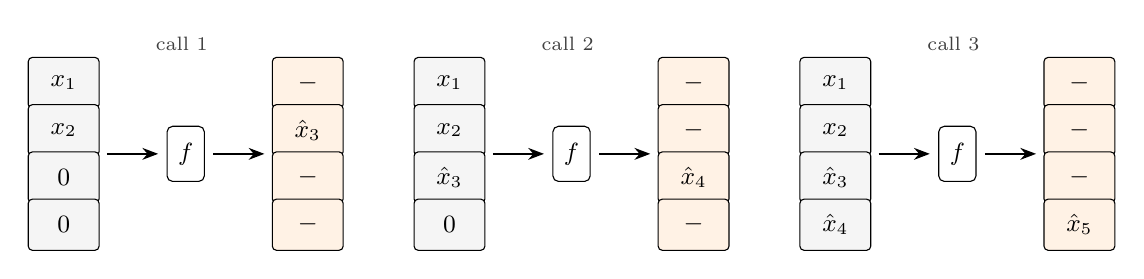
\begin{tikzpicture}
\foreach \s/\ins/\outs in {0/{$x_1$,$x_2$,0,0}/{$-$,$\hat x_3$,$-$,$-$}, 1/{$x_1$,$x_2$,$\hat x_3$,0}/{$-$,$-$,$\hat x_4$,$-$}, 2/{$x_1$,$x_2$,$\hat x_3$,$\hat x_4$}/{$-$,$-$,$-$,$\hat x_5$}}{
 \begin{scope}[xshift=\s*4.9cm]
 \foreach \t [count=\r from 0] in \ins {\node[tok,minimum width=9mm,fill=gray!8] at (0,-\r*0.6) {\t};}
 \node[box] at (1.55,-0.9) {$f$};
 \draw[arr] (0.55,-0.9)--(1.2,-0.9); \draw[arr] (1.9,-0.9)--(2.55,-0.9);
 \foreach \t [count=\r from 0] in \outs {\node[tok,minimum width=9mm,fill=orange!10] at (3.1,-\r*0.6) {\t};}
 \end{scope}}
\node[lbl] at (1.5,0.5) {call 1}; \node[lbl] at (6.4,0.5) {call 2}; \node[lbl] at (11.3,0.5) {call 3};
\end{tikzpicture}
\caption{Autoregressive forecasting with a window of $n=4$: at each call the output at the last observed position is the new prediction (orange), which is appended to the input of the next call. Original redrawing of the example on slide 49.}
\end{figure}

\subsection{Autoregressive generation}\slides{50}
\begin{figure}[H]
\centering
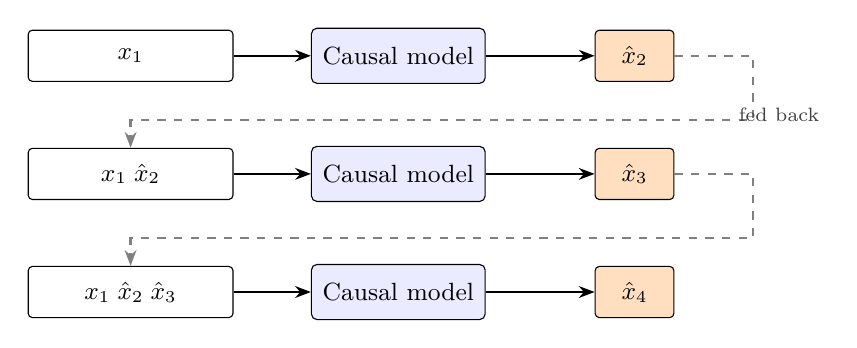
\begin{tikzpicture}
\foreach \r/\ins/\newt in {0/{$x_1$}/{$\hat x_2$}, 1/{$x_1\;\hat x_2$}/{$\hat x_3$}, 2/{$x_1\;\hat x_2\;\hat x_3$}/{$\hat x_4$}}{
 \node[tok,minimum width=26mm] (in\r) at (0,-\r*1.5) {\ins};
 \node[box,fill=blue!8] (m\r) at (3.4,-\r*1.5) {Causal model};
 \node[tok,fill=orange!25,minimum width=10mm] (o\r) at (6.4,-\r*1.5) {\newt};
 \draw[arr] (in\r)--(m\r); \draw[arr] (m\r)--(o\r);
}
\draw[arr,dashed,gray] (o0.east) -- ++(1.0,0) |- ($(in1.north)+(0,0.35)$) -- (in1.north);
\draw[arr,dashed,gray] (o1.east) -- ++(1.0,0) |- ($(in2.north)+(0,0.35)$) -- (in2.north);
\node[lbl,anchor=west] at (7.6,-0.75) {fed back};
\end{tikzpicture}
\caption{Autoregressive generation: the (causal) model is called recursively, each time on a longer input; each new prediction (orange) is appended to the input of the next call. Redrawn from slide 50 (the gray padding of the slide is omitted).}
\end{figure}

\subsection{Causal models}\slides{51}
For a model to perform autoregression, its operations must be \emph{causal}.

\begin{definition}[Causal model]
For a temporal sequence $X\in\R^{n\times c}$, a model $H=f(X)\in\R^{n\times c'}$ is \emph{causal} if $[H]_i$ depends only on $[X]_j$ for $j\le i$.
\end{definition}
In this way the information on the token being generated cannot come from future (not-yet-generated) tokens.

\subsection{Building a causal transformer}\slides{52}
To build a causal variant we replace the SA layer with a \textbf{masked} variant.

\begin{definition}[Masked self-attention]
\[
H=\softmax\!\Big(\frac{QK^\top+M}{\sqrt q}\Big)V,\qquad M_{ij}=\begin{cases}0&\text{if }j\le i,\\-\infty&\text{otherwise.}\end{cases}
\]
In the slides this is written with an element-wise product, $QK^\top\odot M$, and a mask with entries $1$ and $-\infty$; the intended meaning is ``keep the scores with $j\le i$ and replace the others by $-\infty$'', which is what the additive form above computes. In practice we use a very \emph{large negative} number (e.g.\ $-10^{10}$) instead of $-\infty$.
\end{definition}

\begin{proposition}[Masked attention is causal]\label{prop:causal}
Masked SA, and hence a transformer block whose other operations (LN, MLP, residuals) act on each row separately, is causal. A stack of such blocks with positional embeddings is causal.
\end{proposition}
\begin{proof}
For $j>i$ the mask gives $e^{-\infty}=0$, so $a_{ij}=0$ and $h_i=\sum_{j\le i}a_{ij}v_j$ depends only on $x_j$, $j\le i$. Row-wise operations keep this property, and a composition of causal maps is causal.
\end{proof}

\begin{intuition}
During training we want to predict every next token \emph{in parallel} from one long sentence. The mask is a ``blindfold for the future'': token $i$ may look at itself and the past, never at what it is supposed to predict. Otherwise the model would just copy the answer.
\end{intuition}

\subsection{Visualizing the masking operation}\slides{53}
\begin{example}[Masking, step by step]\label{ex:mask}
Let the unmasked scores of four tokens be
\[
S=\begin{pmatrix}1&0.5&-0.5&2\\0&1.5&1&-1\\0.5&0&2&1\\-1&1&0.5&1.5\end{pmatrix}.
\]
After masking (upper triangle $\to-\infty$) and softmax the attention matrix is
\[
A=\begin{pmatrix}1&0&0&0\\0.18&0.82&0&0\\0.16&0.10&0.74&0\\0.04&0.30&0.18&0.49\end{pmatrix}.
\]
Row 1 can only attend to itself, row 4 sees everything.
\end{example}

\begin{figure}[H]
\centering
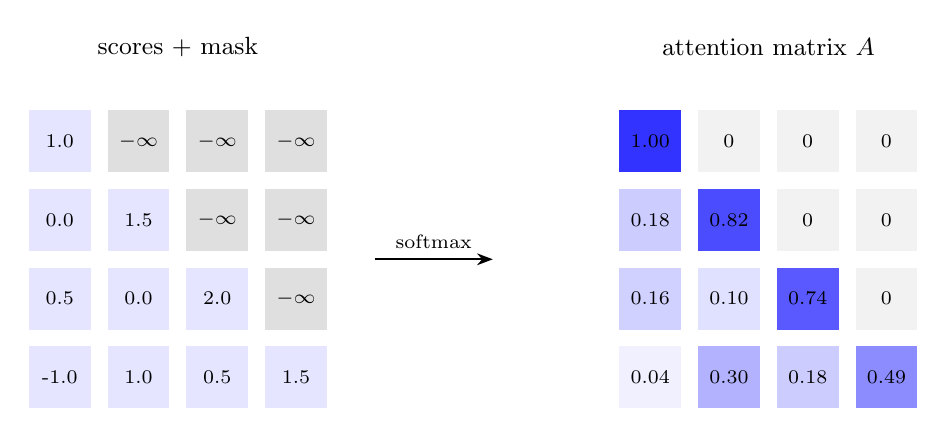
\begin{tikzpicture}[c/.style={minimum size=8mm,inner sep=0,font=\scriptsize,draw=white}]
% scores + mask
\begin{scope}
\def\mm{-}
\foreach \r/\c/\v in {1/1/1.0,1/2/-,1/3/-,1/4/-,2/1/0.0,2/2/1.5,2/3/-,2/4/-,3/1/0.5,3/2/0.0,3/3/2.0,3/4/-,4/1/-1.0,4/2/1.0,4/3/0.5,4/4/1.5}{
 \ifx\v\mm\node[c,fill=gray!25] at (\c,-\r) {$-\infty$};\else\node[c,fill=blue!10] at (\c,-\r) {\v};\fi}
\node[font=\small] at (2.5,0.2) {scores $+$ mask};
\end{scope}
\draw[arr] (5.0,-2.5)--node[above,font=\scriptsize]{softmax}(6.5,-2.5);
\begin{scope}[xshift=7.5cm]
\foreach \r/\c/\v/\p in {1/1/1.00/80,2/1/0.18/20,2/2/0.82/70,3/1/0.16/18,3/2/0.10/12,3/3/0.74/65,4/1/0.04/6,4/2/0.30/30,4/3/0.18/20,4/4/0.49/45}{
 \node[c,fill=blue!\p!white] at (\c,-\r) {\v};}
\foreach \r/\c in {1/2,1/3,1/4,2/3,2/4,3/4}{\node[c,fill=gray!10] at (\c,-\r) {0};}
\node[font=\small] at (2.5,0.2) {attention matrix $A$};
\end{scope}
\end{tikzpicture}
\caption{Masking the upper triangle with $-\infty$ \emph{before} the softmax gives a lower-triangular, row-normalized matrix. Masking with $0$ is invalid because $\exp(0)=1$ still contributes; masking \emph{after} the softmax is invalid because the rows would no longer sum to one (the denominator would still include the future). Numbers from Example~\ref{ex:mask}.}
\end{figure}

\subsection{Cross-attention}\slides{54}
\begin{definition}[Cross-attention]
Given two sets $X$ (e.g.\ $n_X$ tokens) and $Z$ ($n_Z$ tokens),
\begin{equation}\label{eq:cross}
\CA(X,Z)=\softmax\!\Big(\frac{(ZW_q)(XW_k)^\top}{\sqrt q}\Big)XW_v\ \in\R^{n_Z\times v}.
\end{equation}
Queries come from $Z$, keys and values from $X$ (the slide omits the scaling factor).
\end{definition}
This is a useful operation to combine information from different streams (e.g.\ audio-visual datasets).

\begin{proposition}
$\CA(X,X)=\SA(X)$ with shared weights, and the output has as many rows as $Z$ regardless of $n_X$.
\end{proposition}

\begin{intuition}
In self-attention a sequence ``talks to itself''. In cross-attention one stream (e.g.\ the sentence being written in French) \emph{asks questions} and another stream (the English sentence that was encoded) \emph{provides the answers}: the French words look up which English words are relevant to them.
\end{intuition}

\subsection{Full encoder-decoder architecture}\slides{55}
\begin{figure}[H]
\centering
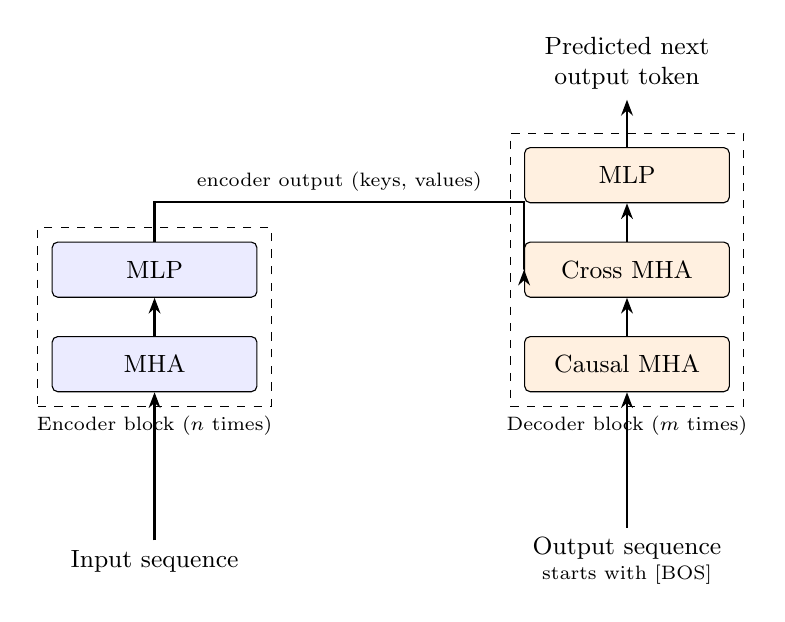
\begin{tikzpicture}[blk/.style={draw,rounded corners=2pt,minimum height=7mm,minimum width=26mm,inner sep=3pt,font=\small,align=center}]
% encoder
\node[blk,fill=blue!8] (e1) at (0,0) {MHA};
\node[blk,fill=blue!8] (e2) at (0,1.2) {MLP};
\node[draw,dashed,fit=(e1)(e2),inner sep=5pt,label={[font=\scriptsize]below:Encoder block ($n$ times)}] {};
\node[font=\small] (in) at (0,-2.5) {Input sequence};
\draw[arr] (in)--(e1.south); \draw[arr] (e1)--(e2);
% decoder
\node[blk,fill=orange!12] (d1) at (6,0) {Causal MHA};
\node[blk,fill=orange!12] (d2) at (6,1.2) {Cross MHA};
\node[blk,fill=orange!12] (d3) at (6,2.4) {MLP};
\node[draw,dashed,fit=(d1)(d2)(d3),inner sep=5pt,label={[font=\scriptsize]below:Decoder block ($m$ times)}] {};
\node[font=\small,align=center] (out) at (6,-2.5) {Output sequence\\[-2pt]{\scriptsize starts with [BOS]}};
\draw[arr] (out)--(d1.south); \draw[arr] (d1)--(d2); \draw[arr] (d2)--(d3);
\draw[arr] (e2.north) -- ++(0,0.5) -| node[pos=0.25,above,font=\scriptsize]{encoder output (keys, values)} (d2.west |- 3.0,1.2) -- (d2.west);
\draw[arr] (d3.north) -- ++(0,0.6) node[above,font=\small,align=center] {Predicted next\\output token};
\end{tikzpicture}
\caption{Encoder-decoder transformer. The encoder processes the full input with (unmasked) MHA; the decoder uses causal MHA on the tokens generated so far, cross-attention to the encoder output, and an MLP. Redrawn from slide 55; residuals and LN omitted.}
\end{figure}

\begin{algorithm}[Autoregressive decoding]\label{alg:decode}
\textbf{Input:} input sequence $x$; trained encoder and decoder; maximum length $T$.
\begin{enumerate}[nosep]
\item $Z\leftarrow\mathrm{Encoder}(x)$.
\item $y\leftarrow[\mathrm{BOS}]$.
\item \textbf{for} $t=1,\dots,T$: compute $p\leftarrow\mathrm{Decoder}(y,Z)$ and take the distribution at the last position; choose the next token $y_t$ (argmax or sampling); \textbf{if} $y_t=\mathrm{EOS}$ \textbf{stop}; else append $y_t$ to $y$.
\item \textbf{return} $y$.
\end{enumerate}
\end{algorithm}

\begin{intuition}
Translation recipe: the encoder reads the whole French sentence once and produces a ``memory'' $Z$. The decoder then writes English one word at a time; each new word looks at the English written so far (causal self-attention) and at the French memory (cross-attention) before choosing the next word, until it writes ``end of sentence''.
\end{intuition}

%==========================================================
\section{Computational considerations}\slides{56--59}

\subsection{Comparing convolutive layers and MHA layers}\slides{56}
\begin{figure}[H]
\centering
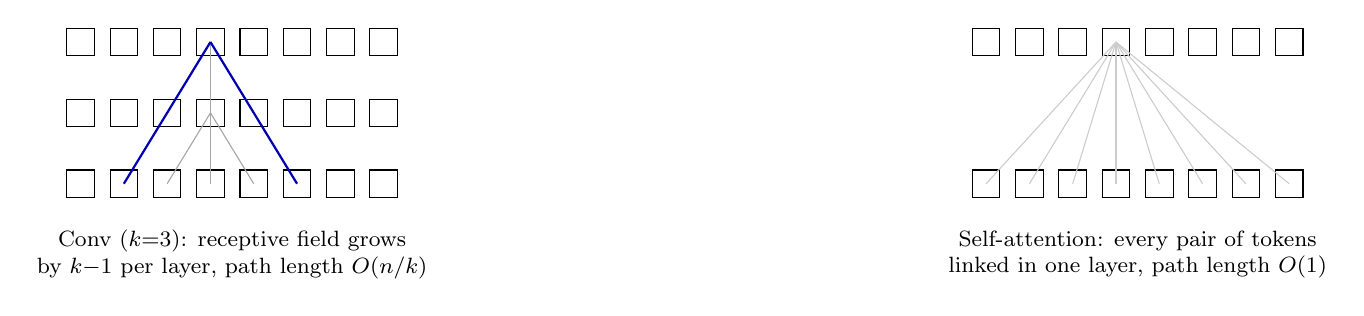
\begin{tikzpicture}[x=0.55cm,y=0.9cm]
\newcommand{\tokrow}[1]{\foreach \i in {1,...,8}{\node[draw,minimum size=3.5mm,inner sep=0] at (\i,#1) {};}}
\begin{scope}
\tokrow{0}\tokrow{1}\tokrow{2}
\foreach \y in {0,1}{\foreach \i in {3,4,5}{\draw[gray!70] (4,\y+1)--(\i,\y);}}
\foreach \i in {3,4,5}{\draw[gray!70] (4,2)--(\i,1);}
\draw[blue!70!black,thick] (4,2)--(3,1)--(2,0); \draw[blue!70!black,thick] (4,2)--(5,1)--(6,0);
\node[font=\footnotesize,align=center] at (4.5,-1) {Conv ($k{=}3$): receptive field grows\\ by $k{-}1$ per layer, path length $O(n/k)$};
\end{scope}
\begin{scope}[xshift=11.5cm]
\tokrow{0}\tokrow{2}
\foreach \i in {1,...,8}{\draw[gray!40] (4,2)--(\i,0);}
\node[font=\footnotesize,align=center] at (4.5,-1) {Self-attention: every pair of tokens\\ linked in one layer, path length $O(1)$};
\end{scope}
\end{tikzpicture}
\caption{Original sketch for the comparison on slide 56 (which reproduces a figure from Chapter 10.6 of \emph{Dive into Deep Learning}): information from a distant token reaches the output after many convolutional layers, but in a single attention layer.}
\end{figure}

\subsection{Computational cost comparison}\slides{57}
\begin{proposition}[Cost of Conv1D vs.\ SA]\label{prop:cost}
Let $X\in\R^{n\times d}$.
\begin{itemize}[nosep]
\item A Conv1D with filter size $k$, $d$ input and $d$ output channels needs $O(nkd^2)$ operations, and has receptive field $k$.
\item A single-head SA layer needs $O(nd^2)$ for the projections $Q,K,V$ and $O(n^2d)$ for $QK^\top$ and for $AV$: $O(nd^2+n^2d)$ in total; the receptive field of a single layer is $n$.
\end{itemize}
\end{proposition}
\begin{proof}
Conv1D: each of the $n$ outputs is a sum of $k$ products of a $d\times d$ matrix by a $d$-vector ($d^2$ operations each). SA: three products $(n\times d)(d\times q)$ cost $O(ndq)=O(nd^2)$; $QK^\top$ is $(n\times q)(q\times n)$, i.e.\ $O(n^2q)$; $AV$ is $(n\times n)(n\times v)$, i.e.\ $O(n^2v)$.
\end{proof}

\begin{example}\label{ex:cost}
$n=1024$, $d=512$, $k=3$. Conv: $nkd^2\approx8.1\cdot10^8$. SA: $3nd^2\approx8.1\cdot10^8$ for the projections and $n^2d\approx5.4\cdot10^8$ for the scores (the same for $AV$). The two terms are equal when $n=d$; for $n\gg d$ the quadratic term dominates.
\end{example}

\begin{table}[ht]
\centering\small
\begin{tabular}{@{}lccc@{}}
\toprule
Layer & Cost per layer & Max.\ path length & Receptive field (1 layer)\\
\midrule
Conv1D (filter $k$) & $O(nkd^2)$ & $O(n/k)$ layers & $k$\\
Self-attention & $O(nd^2+n^2d)$ & $O(1)$ & $n$\\
\bottomrule
\end{tabular}
\caption{Conv1D vs.\ self-attention. Path length: number of layers needed to connect two tokens at distance $n$ (standard $D2L$-style comparison, consistent with the slide).}
\end{table}

\begin{intuition}
Attention buys you ``see everything at once'' at the price of a bill that grows with the \emph{square} of the sequence length. Doubling $n$ doubles the cost of a convolution, but quadruples the attention term. The $n^2$ term is why long sequences are the main practical bottleneck, although very efficient implementations and hardware (e.g.\ FlashAttention) are available today.
\end{intuition}

\subsection{Memory considerations}\slides{58}
Materializing the $QK^\top$ matrix also requires $O(n^2)$ \emph{memory}. Modern implementations (e.g.\ FlashAttention) avoid this by processing the tokens in multiple \emph{chunks}: they store intermediate values for the softmax denominator and only apply the normalization at the end (\textbf{lazy softmax}).

\begin{example}
$n=8192$ in 16-bit precision: $8192^2\cdot2$ bytes $=128$ MiB \emph{per head, per layer, per sequence} just for the score matrix.
\end{example}

\begin{algorithm}[Lazy (online) softmax attention for one query]\label{alg:lazy}
Query $q_i$; keys/values processed in chunks $\mathcal C_1,\dots,\mathcal C_B$. Maintain a running maximum $\mu$, a running denominator $\ell$ and a running vector $u$; start with $\mu=-\infty$, $\ell=0$, $u=0$.
\begin{enumerate}[nosep]
\item For each chunk $b$: compute $s_j=q_i^\top k_j/\sqrt q$ for $j\in\mathcal C_b$; $\mu'=\max(\mu,\max_js_j)$.
\item Rescale: $\ell\leftarrow e^{\mu-\mu'}\ell+\sum_je^{s_j-\mu'}$; $u\leftarrow e^{\mu-\mu'}u+\sum_je^{s_j-\mu'}v_j$; $\mu\leftarrow\mu'$.
\item After the last chunk return $h_i=u/\ell$.
\end{enumerate}
\end{algorithm}

\begin{proposition}
Algorithm~\ref{alg:lazy} returns exactly $h_i=\sum_j\softmax_j(s)\,v_j$, while keeping only one chunk of scores in memory.
\end{proposition}
\begin{proof}
Invariant: after processing chunks $1..b$, $\ell=\sum_{j\in\mathcal C_{\le b}}e^{s_j-\mu}$ and $u=\sum_{j\in\mathcal C_{\le b}}e^{s_j-\mu}v_j$, with $\mu$ the maximum score so far. It holds initially and the rescaling by $e^{\mu-\mu'}$ changes the reference point from $\mu$ to $\mu'$. At the end $u/\ell=\sum_je^{s_j-\mu}v_j/\sum_je^{s_j-\mu}$, which is the softmax-weighted average (the constant $e^{-\mu}$ cancels).
\end{proof}

\begin{intuition}
You never need the whole $n\times n$ table at once: read the keys chunk by chunk, keep a running ``sum so far'' and fix it up (rescale) whenever you meet a new, larger score. The normalization is applied once at the end, hence \emph{lazy} softmax.
\end{intuition}

\subsection{KV Cache}\slides{59}
The KV cache is an essential component of autoregressive implementations (see the book).

\begin{proposition}[Cached keys and values do not change]
In a causal transformer, $k_j$ and $v_j$ of token $j$ at every layer depend only on tokens $\le j$ (Proposition~\ref{prop:causal}). Hence when a new token $t$ is appended, keys and values of tokens $1,\dots,t-1$ are unchanged and can be stored. Generating token $t$ then needs only the projections of the new token and attention of its query against the cache: $O(d^2+td)$ per layer, instead of $O(td^2+t^2d)$.
\end{proposition}

\begin{figure}[H]
\centering
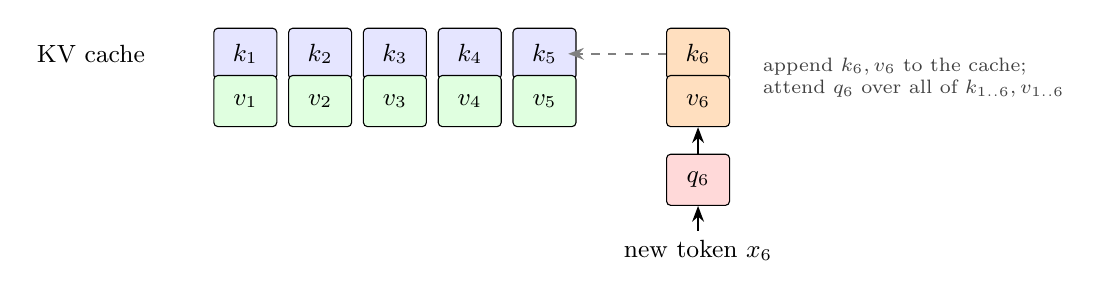
\begin{tikzpicture}
\node[font=\small,anchor=east] at (-0.2,1.2) {KV cache};
\foreach \i in {1,...,5}{
 \node[tok,fill=blue!10,minimum width=8mm] at (\i*0.95,1.2) {$k_\i$};
 \node[tok,fill=green!12,minimum width=8mm] at (\i*0.95,0.6) {$v_\i$};}
\node[tok,fill=orange!25,minimum width=8mm] (nk) at (6.7,1.2) {$k_6$};
\node[tok,fill=orange!25,minimum width=8mm] (nv) at (6.7,0.6) {$v_6$};
\node[tok,fill=red!15,minimum width=8mm] (nq) at (6.7,-0.4) {$q_6$};
\node[font=\small] (nx) at (6.7,-1.3) {new token $x_6$};
\draw[arr] (nx)--(nq); \draw[arr] (nq.north)--(nv.south);
\draw[arr,dashed,gray] (nk.west) -- (5.05,1.2);
\node[lbl,align=left,anchor=west] at (7.4,0.9) {append $k_6,v_6$ to the cache;\\attend $q_6$ over all of $k_{1..6},v_{1..6}$};
\end{tikzpicture}
\caption{KV cache: only the new token's $q,k,v$ are computed; old keys/values are read from memory. Original redrawing of slide 59.}
\end{figure}

\begin{example}
Generating $T$ tokens without cache costs $\sum_{t\le T}O(td^2+t^2d)=O(T^2d^2+T^3d)$; with cache $\sum_tO(d^2+td)=O(Td^2+T^2d)$. The price is memory: $2\cdot t\cdot m$ numbers per layer, which is why multi-query attention (a factor $h$ smaller cache) is attractive.
\end{example}

\begin{intuition}
Don't re-read the whole book to write the next word. Keep notes (keys and values) on everything already read; the only new work is reading the notes with the single new question.
\end{intuition}

%==========================================================
\section{Practical transformer models}\slides{60--65}

\subsection{Text transformers: transformers for contextual embeddings}\slides{60}
The majority of pre-trained word embedding models are standard transformer models trained on the sequence of text tokens.
\begin{itemize}[nosep]
\item \textbf{BERT-like} models are pre-trained by masking one word in a sentence and reconstructing the full sentence in output.
\item \textbf{GPT-like} models are (causal) variants pre-trained to generate the sequence autoregressively.
\end{itemize}
These are called \emph{contextual embeddings} because the same word in different sentences can be encoded into different vectors.

\begin{definition}[Pre-training objectives]
BERT-like (masked language modelling): maximize $\sum_{t\in\mathcal M}\log p(x_t\mid x_{\setminus\mathcal M})$ over the masked positions $\mathcal M$. GPT-like (causal language modelling): maximize $\sum_{t=1}^{n}\log p(x_t\mid x_{<t})$, which by Proposition~\ref{prop:chain} is the exact log-likelihood of the sequence.
\end{definition}

\begin{example}
``I sat on the river \underline{bank}'' vs.\ ``I deposited cash at the \underline{bank}'': a one-hot or trainable (static) embedding gives the same vector for ``bank''; a transformer produces two different vectors because its representation of the token is a function of its attention over the rest of the sentence.
\end{example}

\subsection{Self-supervised learning}\slides{61}
Because these models are trained from raw text alone (no specific targets), they are called \textbf{self-supervised} (to be covered in depth later). Their strength is that scaling laws for transformers are empirically better than for other models, i.e.\ they benefit more from increasing the dataset by orders of magnitude. In NLP this is also shown by the emergence of paradigms like text-prompting and zero-shot learning.

\begin{intuition}
The labels come for free: in a sentence, the ``answer'' for token $t$ is just the next word. With a huge text corpus there is an essentially unlimited supply of training examples.
\end{intuition}

\subsection{Vision transformers: applying transformers on images}\slides{62}
Transformers can also benefit computer vision, especially when trained on huge datasets (e.g.\ ImageNet-21k). However, this requires converting the original image (a 2D grid) into a 1D sequence (actually a \emph{set}, together with positional embeddings). Because using pixels would scale quadratically in the number of pixels, a common solution is to work on \textbf{patches} of the image.

\begin{definition}[Patch embedding]
An image $I\in\R^{H\times W\times C}$ is cut into $N=HW/P^2$ non-overlapping $P\times P$ patches; each is flattened to a vector of size $P^2C$ and linearly projected to $\R^d$. A class token and positional embeddings are added, and the sequence goes through a standard transformer.
\end{definition}

\begin{example}
$224\times224$ images with $P=16$: $N=14^2=196$ tokens, so the attention matrix has $196^2\approx3.8\cdot10^4$ entries. With one token per pixel it would have $(224^2)^2\approx2.5\cdot10^9$ entries, $65{,}000$ times more.
\end{example}

\subsection{Vision Transformer (ViT)}\slides{63}
\begin{figure}[H]
\centering
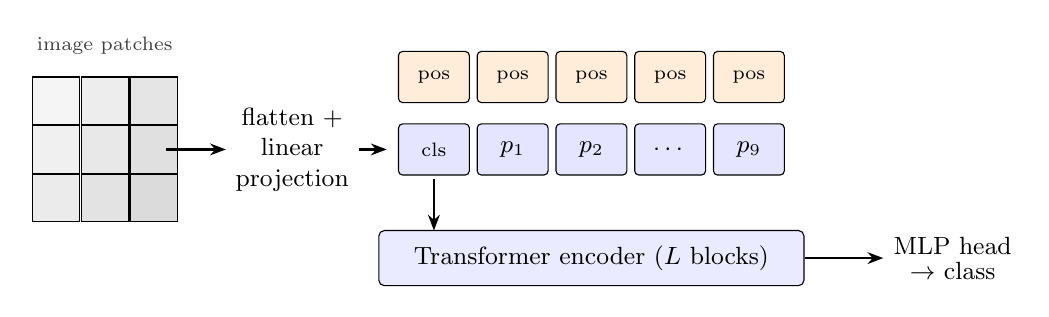
\begin{tikzpicture}
% image with patch grid
\foreach \i in {0,1,2}{\foreach \j in {0,1,2}{
 \node[draw,minimum size=6mm,fill=gray!\the\numexpr 8+\i*6+\j*4\relax] at (\i*0.62,-\j*0.62) {};}}
\node[lbl] at (0.62,0.7) {image patches};
\node[font=\small,align=center] (fl) at (3.0,-0.62) {flatten +\\linear\\projection};
\draw[arr] (1.4,-0.62)--(fl.west);
\foreach \i/\t in {0/{\scriptsize cls},1/{$p_1$},2/{$p_2$},3/{$\cdots$},4/{$p_9$}}{
 \node[tok,minimum width=9mm,fill=blue!10] at (4.8+\i*1.0,-0.62) {\t};
 \node[tok,minimum width=9mm,fill=orange!15] at (4.8+\i*1.0,0.3) {\scriptsize pos};}
\draw[arr] (fl.east)--(4.2,-0.62);
\node[box,fill=blue!8,minimum width=5.4cm] (te) at (6.8,-2.0) {Transformer encoder ($L$ blocks)};
\draw[arr] (4.8,-1.0)--(4.8,-1.65);
\draw[arr] (te.east) -- ++(1.0,0) node[right,font=\small,align=center] {MLP head\\[-2pt]$\to$ class};
\end{tikzpicture}
\caption{ViT: a standard transformer on top of image patches (flattened, projected, plus positional embeddings and a class token). Original schematic of slide 63 (Dosovitskiy et al., 2020).}
\end{figure}

\subsection{Mixer models}\slides{64}
Mixer models are variants of the ViT where the MHA is replaced by fully-connected layers (Tolstikhin et al., 2021).

\begin{definition}[Mixer block]
For a table $X\in\R^{N\times d}$ of $N$ patch tokens: a \emph{token-mixing} MLP acts across patches (on the columns), $U=X+\big(\mathrm{MLP}_1(\LN(X)^\top)\big)^\top$, then a \emph{channel-mixing} MLP acts on each patch separately, $Y=U+\mathrm{MLP}_2(\LN(U))$.
\end{definition}

\begin{figure}[H]
\centering
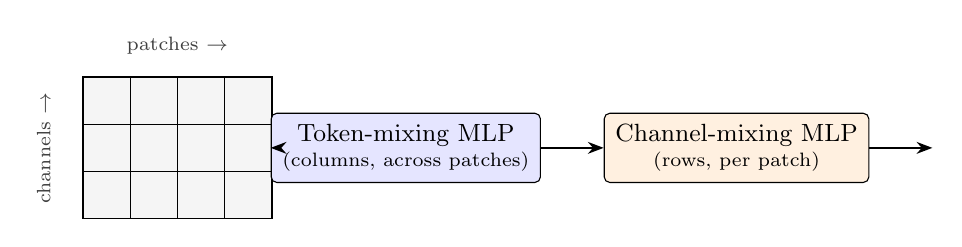
\begin{tikzpicture}
\foreach \i in {1,...,4}{\foreach \j in {1,...,3}{\node[draw,minimum size=6mm,fill=gray!8] at (\i*0.6,-\j*0.6) {};}}
\node[lbl] at (1.5,0.1) {patches $\to$};\node[lbl,rotate=90] at (-0.2,-1.2) {channels $\to$};
\node[box,fill=blue!10] (tm) at (4.4,-1.2) {Token-mixing MLP\\[-2pt]{\scriptsize (columns, across patches)}};
\node[box,fill=orange!12] (cm) at (8.6,-1.2) {Channel-mixing MLP\\[-2pt]{\scriptsize (rows, per patch)}};
\draw[arr] (2.8,-1.2)--(tm.west); \draw[arr] (tm)--(cm); \draw[arr] (cm.east)--++(0.8,0);
\end{tikzpicture}
\caption{Mixer: the same alternation ``mix tokens / update each token'' as a transformer block, but token mixing is a fixed-size MLP instead of attention. Redrawn from slide 64.}
\end{figure}

\begin{intuition}
It tests an interesting question: is it the \emph{attention} that matters, or just the ``mix across tokens, then per token'' structure? The trade-off: the token-mixing MLP has weights tied to a fixed number of patches and positions, while attention weights are computed from the data and work for any $n$.
\end{intuition}

\subsection{Multimodal models}\slides{65}
Transformers also simplify multimodal models by projecting tokens of different modalities into a \textbf{single embedding space}.

\begin{figure}[H]
\centering
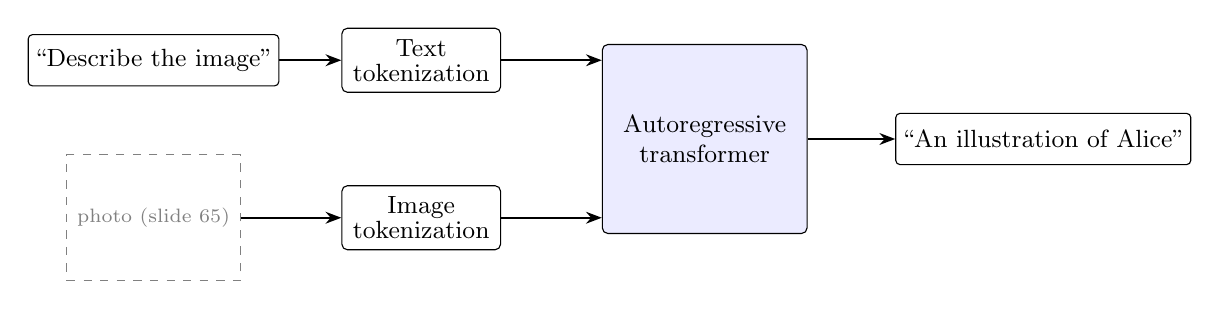
\begin{tikzpicture}
\node[tok,minimum width=30mm] (t) at (0,1.0) {``Describe the image''};
\node[box] (tt) at (3.4,1.0) {Text\\[-2pt]tokenization};
\node[draw,dashed,gray,minimum width=22mm,minimum height=16mm] (im) at (0,-1.0) {\scriptsize photo (slide 65)};
\node[box] (it) at (3.4,-1.0) {Image\\[-2pt]tokenization};
\node[box,fill=blue!8,minimum height=24mm,minimum width=26mm] (tr) at (7.0,0) {Autoregressive\\transformer};
\node[tok,minimum width=34mm] (o) at (11.3,0) {``An illustration of Alice''};
\draw[arr] (t)--(tt); \draw[arr] (im)--(it);
\draw[arr] (tt.east)--(tr.west |- tt.east); \draw[arr] (it.east)--(tr.west |- it.east);
\draw[arr] (tr.east)--(o.west);
\end{tikzpicture}
\caption{Multimodal model: the tokens of different modalities (text and image) form one sequence for a single autoregressive transformer. Original schematic redrawn from slide 65.}
\end{figure}

\begin{figure}[H]
	\centering
	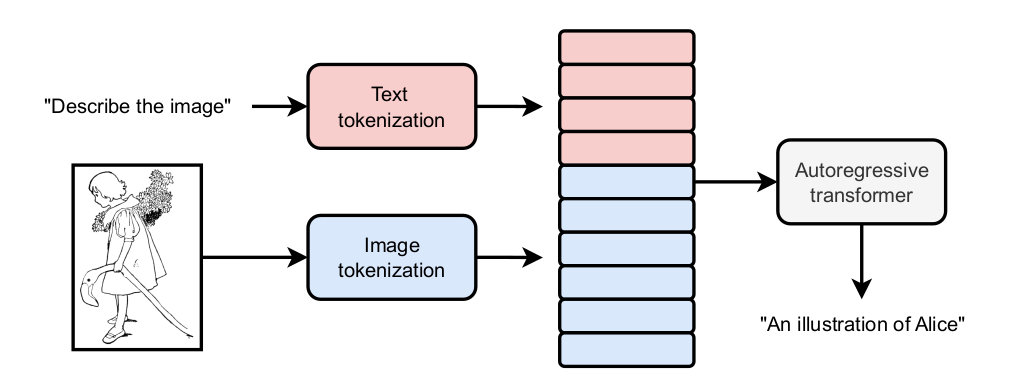
\includegraphics[width=1.0\linewidth]{1795435564889.png}
	\caption{Transformers also simplify multimodal models by projecting tokens of different modalities in a single embedding space.}\label{fig:1795435564889}
\end{figure}
%==========================================================
\section{Summary}

\subsection{Comparison of the layers and models covered}
\begin{table}[H]
\centering\scriptsize
\renewcommand{\arraystretch}{1.25}
\begin{tabular}{@{}p{2.6cm}p{3.3cm}p{2.9cm}p{2.9cm}p{2.6cm}@{}}
\toprule
\textbf{Layer / model} & \textbf{Weight of $x_j$ in $h_i$} & \textbf{Parameters} & \textbf{Cost (time)} & \textbf{Main limitation}\\
\midrule
Conv1D (size $k$) & trainable $W_{j-i}$, only $|j-i|\le k$ & $(2k{+}1)d^2$ & $O(nkd^2)$ & local only\\
Continuous conv. & $g(j-i)$, any offset & size of $g$ & $O(n^2d^2)$ (naive) & depends on offset only\\
Non-local layer & $\alpha(x_i,x_j)$, content-based & depends on $\alpha$ & $O(n^2d)$ & no projections\\
Self-attention & $\softmax_j(q_i^\top k_j/\sqrt q)$ & $d(2q{+}v)$ & $O(nd^2+n^2d)$ & ignores order, $O(n^2)$\\
Multi-head attention & $h$ different softmax maps, mixed by $W_o$ & $3dm+mo$ & same as 1 head & ignores order, $O(n^2)$\\
Masked MHA & as MHA, $a_{ij}=0$ for $j>i$ & same & same & future-blind\\
Cross-attention & queries from $Z$, keys/values from $X$ & same & $O(n_Zn_Xd)$ & needs two streams\\
\bottomrule
\end{tabular}
\caption{The attention family compared to convolutions (continuous-conv.\ cost is for a naive evaluation of $g$ at all offsets).}
\end{table}

\begin{table}[H]
\centering\scriptsize
\renewcommand{\arraystretch}{1.25}
\begin{tabular}{@{}p{2.8cm}p{3.6cm}p{3.6cm}p{3.0cm}@{}}
\toprule
\textbf{Position scheme} & \textbf{Idea} & \textbf{Pros} & \textbf{Cons}\\
\midrule
One-hot / scalar & slot index or $i/p$ & trivial & poor empirically, fixed $p$\\
Trainable & one learned vector per position & flexible & fixed max length (interpolate)\\
Sinusoidal & multi-frequency sin/cos clock & any length, shift $=$ rotation & fixed, absolute\\
ALiBi (relative) & bias $b(i-j)$ on scores & extrapolates to longer inputs & only a distance penalty\\
RoPE (relative) & rotate $q,k$ by position & dot product depends on $j-i$ & implementation detail\\
\bottomrule
\end{tabular}
\caption{Positional schemes seen in the slides.}
\end{table}

\begin{table}[H]
\centering\scriptsize
\renewcommand{\arraystretch}{1.25}
\begin{tabular}{@{}p{2.8cm}p{3.6cm}p{3.6cm}p{3.0cm}@{}}
\toprule
\textbf{Model type} & \textbf{Attention} & \textbf{Training / use} & \textbf{Example}\\
\midrule
Encoder-only & full & contextual embeddings, classification & BERT, ViT\\
Decoder-only (causal) & masked & autoregressive generation, KV cache & GPT\\
Encoder-decoder & full + masked + cross & seq2seq (translation) & original transformer\\
\bottomrule
\end{tabular}
\caption{Three families of transformer models.}
\end{table}

\subsection{A qualitative comparison: cost versus sequence length}
\begin{figure}[H]
\centering
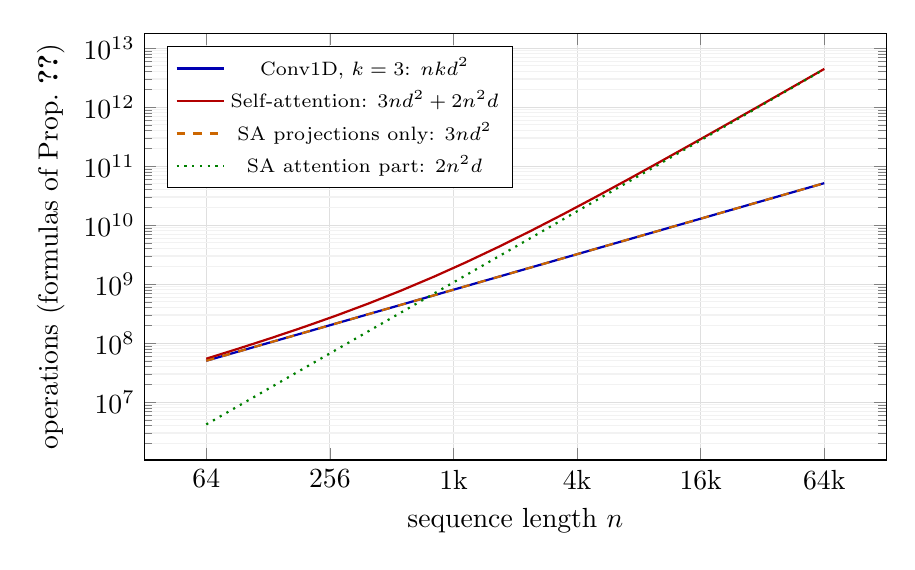
\begin{tikzpicture}
\begin{axis}[width=11cm,height=7cm,xmode=log,ymode=log,log basis x=2,xlabel={sequence length $n$},ylabel={operations (formulas of Prop.~\ref{prop:cost})},
 grid=both,major grid style={gray!25},minor grid style={gray!10},legend pos=north west,legend style={font=\scriptsize},domain=64:65536,samples=20,xtick={64,256,1024,4096,16384,65536},xticklabels={64,256,1k,4k,16k,64k}]
\addplot[thick,blue!70!black] {x*3*512*512};
\addlegendentry{Conv1D, $k=3$: $nkd^2$}
\addplot[thick,red!70!black] {3*x*512*512 + 2*x*x*512};
\addlegendentry{Self-attention: $3nd^2+2n^2d$}
\addplot[thick,dashed,orange!80!black] {3*x*512*512};
\addlegendentry{SA projections only: $3nd^2$}
\addplot[thick,dotted,green!50!black] {2*x*x*512};
\addlegendentry{SA attention part: $2n^2d$}
\end{axis}
\end{tikzpicture}
\caption{Operation counts for $d=512$ (formulas of Proposition~\ref{prop:cost}, constants set to $3$ for the projections and $2$ for $QK^\top$ and $AV$). Convolution is linear in $n$; the attention curve bends upward and overtakes the $nd^2$ term at $n\approx d$. This is a plot of the formulas, not of measured timings.}
\end{figure}

\subsection{Key take-aways}
\begin{itemize}
\item \textbf{Attention replaces locality with content-based soft sparsity.} Each token mixes the value vectors of all tokens with weights $\softmax(q_i^\top k_j/\sqrt q)$; the $\sqrt q$ keeps the softmax out of saturation and multi-head attention lets every token attend to several subsets at once, at constant parameter count.
\item \textbf{A transformer block = ``talk, then think''.} MHA mixes tokens, a row-wise MLP updates each token, with residuals and layer norm (pre-norm is easier to train).
\item \textbf{Attention is permutation equivariant, so order must be injected.} Absolute (trainable or sinusoidal) or relative (ALiBi, RoPE) positional information is added; the sinusoidal choice turns shifts into rotations.
\item \textbf{Masking + autoregression give generative and seq2seq models.} A triangular $-\infty$ mask makes the model causal; cross-attention connects encoder and decoder; the KV cache makes generation affordable.
\item \textbf{The price is $O(n^2)$ time and memory;} modern implementations (chunked lazy softmax) mitigate it, and the same architecture, applied to text tokens, image patches or multimodal tokens, scales better with data than previous models.
\end{itemize}

\end{document}